%Gilmore Space LaTeX template
%
%Rory Kelly ~ 21 Nov 2024
%Needed for ?. Must come before document class
\RequirePackage{pdfmanagement-testphase}
\DeclareDocumentMetadata{}
\documentclass[12pt]{article}

% Page setup
\usepackage[a4paper]{geometry}

% PDF management (to include PDF pages)
\usepackage{pdfpages}

% Table management (for advanced table formatting)
\usepackage{tabu}

% Font handling
\usepackage{mathspec} 
%\usepackage[no-math]{fontspec} 
\usepackage{fontspec} % for font selection and OpenType/TrueType support

\usepackage[english]{babel} 

% Mathematics support
\usepackage{amsmath, amssymb, amsthm, thmtools}

%\usepackage[no-math]{fontspec} 
%\setmainfont{Gentium Plus} 
%\usepackage[italic]{mathastext}

% Input encoding
\usepackage[utf8]{inputenc}

% File-related commands (for working with file paths)
\usepackage[abspath]{currfile} 

% Section and subsection formatting
\usepackage{titlesec}

% Drawing and custom graphics
\usepackage{tikz} 

% Watermark management
\usepackage{eso-pic} 

% Header and footer formatting
\usepackage{fancyhdr} 

% Get total number of pages
\usepackage{lastpage}

% Optional package for total page count (not used here)
% \usepackage{zref-totpages} % gets the total page numbers

% Graphics support
\usepackage{graphicx}
\usepackage{float}
\usepackage{transparent} % for transparent watermark

% Hyperlink support
\usepackage[colorlinks, allcolors=blue]{hyperref}

% Table formatting
\usepackage{longtable}
\usepackage{booktabs}
\usepackage{adjustbox}
\usepackage{multirow}
\usepackage{multicol}
\usepackage{array}
\usepackage{tabularx}

% Color support
\usepackage[table, svgnames, dvipsnames]{xcolor}
\definecolor{lightbeige}{RGB}{255, 239, 204}
\definecolor{green}{RGB}{0, 128, 0}
\definecolor{codegreen}{rgb}{0, 0.6, 0}
\definecolor{codegray}{rgb}{0.5, 0.5, 0.5}
\definecolor{codepurple}{rgb}{0.58, 0, 0.82}
\definecolor{backcolour}{rgb}{0.95, 0.95, 0.92}

% Code formatting
\usepackage{verbatim}
\usepackage{listings}
\lstset{
    backgroundcolor=\color{backcolour},   
    commentstyle=\color{codegreen},
    keywordstyle=\color{magenta},
    numberstyle=\tiny\color{codegray},
    stringstyle=\color{codepurple},
    basicstyle=\ttfamily\footnotesize,
    breakatwhitespace=false,         
    breaklines=true,                 
    captionpos=b,                    
    keepspaces=true,                 
    numbers=left,                    
    numbersep=5pt,                  
    showspaces=false,                
    showstringspaces=false,
    showtabs=false,                  
    tabsize=2
}

% Caption setup for tables
\usepackage{caption}
\captionsetup[table]{skip=2pt}

% Additional useful packages
\usepackage{subfigure}  % for subfigures
\usepackage{lscape}     % for landscape pages
\usepackage{makecell}   % for table cells
\usepackage{rotating}   % for rotating elements
\usepackage{nomencl}    % for nomenclature

% Clever references
\usepackage[nameinlink, capitalize]{cleveref}

% Miscellaneous styling
\usepackage{color,soul}
%\usepackage{stix, bbm, pifont, utfsym, fontawesome, noto}
\usepackage{stix, bbm, pifont, fontawesome, noto}

\usepackage{ulem}

\setmainfont{Arial}[
]
%
\definecolor{AtmoBlue}{HTML}{00aeef}
\definecolor{DeepSpace}{HTML}{0c004b}
\definecolor{Rocket}{HTML}{c9cacc}
\definecolor{Titles}{HTML}{2f5496}
\definecolor{Table_Light}{HTML}{deeaf6}
\definecolor{Table_Dark}{HTML}{bdd6ee}
\definecolor{Table_Title}{HTML}{5b9bd5}
%
\titleformat{\section}
{\color{Titles}\normalfont\Large}
{\color{Titles}\thesection}{1em}{}
\titleformat{\subsection}
{\color{Titles}\normalfont\large}
{\color{Titles}\thesubsection}{1em}{}
\titleformat{\subsubsection}
{\color{Titles}\normalfont}
{\color{Titles}\thesubsubsection}{1em}{}
%
%%%%%%%%%%%%%%%%%%%%%%%%%%%%%%%%%%%%%%%%%%%%%%%%%%%%%%%%%%%%%%%%%%%%%%%
%%%%%%%%%%%%%%%%%%%%%%%%%%%%%%%%%%%%%%%%%%%%%%%%%%%%%%%%%%%%%%%%%%%%%%%
%%%%%%%%%%%%%%%%%%%%%%%%%%%%%%%%%%%%%%%%%%%%%%%%%%%%%%%%%%%%%%%%%%%%%%%
%
% IMPORTANT, PUT THE DOCUMENT INFORMATION HERE!!!
\newcommand{\DocumentID}{000-00000}
\newcommand{\VersionID}{ABCD}
\newcommand{\PublishID}{\today}
%
\pagestyle{fancy}
\lhead{\scriptsize CHARON Aerodynamics}
\rhead{\scriptsize \DocumentID \\ \VersionID}
\chead{
\includegraphics[width=4cm]{logo.png}}
\lfoot{}
\rfoot{\scriptsize Page \thepage\ of \pageref{LastPage}}
\cfoot{\scriptsize Private and Confidential © 2024 Gilmour Space}
\renewcommand{\headrulewidth}{0.2pt}
\renewcommand{\footrulewidth}{0.2pt}
% LC: prolongate header and foot line
\renewcommand{\headrule}{\hrule width \textwidth} 
\renewcommand{\footrule}{\hrule width \textwidth} 

%
\geometry{
    a4paper,
    total={170mm,257mm},
    margin=1in,
}
%
% \pagenumbering{Roman}
%
%Turn of the LaTeX indents
\setlength{\parindent}{0pt}
\setlength{\parskip}{5pt}
 %
%Totally forgot what this was for
\makeatletter
\setlength{\@fptop}{0pt}
\makeatother
%
%Add the title page background
\AddToShipoutPictureBG*{
    \put(0,0){
        \parbox[b][\paperheight]{\paperwidth}{%
            \vfill
            \centering
            \transparent{0.25}
\includegraphics[width=15cm]{./background.png}%
            \vfill
        }
    }
}

\title{Jet-ON validation test case: Ladenburg jet}
\author{Lorenzo Campoli}
\date{\today}

\begin{document}

\setmainfont{Arial}

\maketitle

\renewcommand{\arraystretch}{1.5} % Adjust row height
\setlength{\tabcolsep}{8pt}       % Adjust column spacing

\begin{center}
\resizebox{\textwidth}{!}{ % Automatically adjust table width to fit the page
\begin{tabular}{m{3.5cm}|m{5cm}m{6.5cm}m{4.5cm}}
%
                      & \textbf{NAME}           & \textbf{TITLE/ROLE} & \textbf{SIGNATURE} \\ \hline
\textbf{AUTHORED BY}  & Lorenzo Campoli         & Senior System Modelling Engineer    & 
\includegraphics[width=4cm]{signature/signature0.png} \\  
\textbf{REVIEWED BY}  & Jonathan Healy          & System Modelling Engineer           & \\ 
                      & Matthew Pengelly        & Senior System Modelling Engineer    & \\ 
\textbf{APPROVED BY}  & Smritee Darcy           & Lead System Mechanical Engineer     & \\
                      & Eleazar Gonzalez-Casas  & Chief Engineer                      & \\ \hline
\end{tabular}}
\end{center}

\begin{abstract}
\noindent In this work package, a validation test case for the jet-on configuration was numerically investigated. The Ladenburg jet test case was selected for this purpose as detailed in the body of the report. The main objective was to build up confidence in the numerical solutions obtained by OpenFOAM and FLUENT solvers for jet-dominated flows. Consequently, the simulation of Charon jet-on configuration can be approached with \textit{trust}. 
\end{abstract}

%\newpage
%\makenomenclature
%\newpage
%\printnomenclature
%\section*{List of Abbreviations}
\begin{tabbing}
    \hspace{3cm} \= \hspace{8cm} \kill
    \textbf{Abbreviation} \> \textbf{Description} \\
    AEDB \> Aerodynamic DataBase  \\
    AF \> Ansys Fluent \\
    AMR \> Adaptive Mesh Refinement \\
    ARCAS \> All-Purpose Rocket for Collecting Atmospheric Soundings \\
    CAD \> Computer Aided Design \\
    CFD \> Computational Fluid Dynamics \\
    ESI \> OpenFOAM ESI Group \\
    FOs \> Functional Objects \\
    GR \> Growth Ratio \\
    GUI \> Graphical User Interface \\
    LTS \> Local Time Stepping \\
    LV \> Launch Vehicle \\
    NASA \> National Aeronautics and Space Administration \\
    OF \> OpenFOAM \\
    OS \> Operating System \\
    PIFS \> Plume-Induced Flow Separation \\
    PISO \> Pressure Implicit with Splitting of Operators \\
    SA \> Spalart Allmaras 1-Equation Turbulence Model \\
    SHM \> snappyHexMesh \\
    SIMPLE \> Semi-Implicit Method for Pressure Linked Equations \\
    SST \> Shear-Stress Transport 2-Equation Turbulence Model \\
    VSC \> Visual Studio Code \\
    WSL \> Windows Subsystem for Linux \\
    CG \> Center of Gravity \\
    CP \> Center of Pressure \\
    LE \> Leading Edge \\
    MAC \> Mean Aerodynamic Chord \\
    RK4 \> Runge-Kutta 4 Integration Method \\
    UI \> User Interface
\end{tabbing}
%
\section*{List of Symbols}
\begin{tabbing}
    \hspace{3cm} \= \hspace{9cm} \= \hspace{9cm} \kill
    \textbf{Sign} \> \textbf{Description} \> \textbf{Unit} \\
    $A$ \> Area \> m$^2$ \\
    $A_{fin}$ \> Area of one fin \> m$^2$ \\
    $A_{plan}$ \> Planform Area \> m$^2$ \\
    $A_{ref}$ \> Reference Area \> m$^2$ \\
    $A_{wet}$ \> Wetted Area \> m$^2$ \\
    $A_{aspect}$ \> Aspect Ratio of a fin, $2s / A_{fin}$ \> - \\
    $c$ \> Speed of Sound \> m/s \\
    $\bar{c}$ \> Mean Aerodynamic Chord Length of a fin \> m \\
    $c(y)$ \> Chord Length of a fin at spanwise position $y$ \> m \\
    $C_A$ \> Aerodynamic Axial Coefficient \> - \\
    $C_N$ \> Aerodynamic Normal Coefficient \> - \\
    $C_m$ \> Pitch Moment Coefficient \> - \\
    $C_{m\alpha}$ \> Pitch Moment Coefficient Derivative, $\frac{\partial C_m}{\partial \alpha}$ \> - \\
    $C_D$ \> Drag Force Coefficient \> - \\
    $C_f$ \> Skin Friction Drag Coefficient \> - \\
    $C_l$ \> Roll Moment Coefficient \> - \\
    $C_{ld}$ \> Roll Damping Moment Coefficient \> - \\
    $C_{lf}$ \> Roll Forcing Moment Coefficient \> - \\
    $D$ \> Hydraulic Diameter \> m \\
    $d$ \> Reference Length (Rocket Diameter) \> m \\
    $f_B$ \> Rocket Fineness Ratio, $L/d$ \> - \\
    $L$ \> Rocket Length \> m \\
    $m$ \> Pitch Moment \> N·m \\
    $N$ \> Normal Force or Number of Fins \> N or - \\
    $p$ \> Air Pressure \> Pa \\
    $Re$ \> Reynolds Number \> - \\
    $s$ \> Spanwise Length of One Fin \> m \\
    $T$ \> Air Temperature \> K \\
    $V$ \> Volume \> m$^3$ \\
    $v_0$ \> Free-Stream Velocity \> m/s \\
    $x$ \> Position Along the Rocket Centerline \> m \\
    $y$ \> Spanwise Position \> m \\
    $\alpha$ \> Angle of Attack \> deg \\
    $\gamma$ \> Specific Heat Ratio (for air, $\gamma = 1.4$) \> - \\
    $\Gamma_c$ \> Fin Midchord Sweep Angle \> deg \\
    $\delta_{fin}$ \> Fin Cant Angle \> deg \\
    $\eta$ \> Airflow Inclination Angle Over a Fin \> deg \\
    $\theta$ \> Roll Angle \> deg \\
    $\Lambda$ \> Dihedral Angle Fin - flow direction \> deg \\
    $\nu$ \> Kinematic Viscosity of Air \> m$^2$/s \\
    $\omega_{vel}$ \> Angular Velocity \> rad/s \\
    %$|M^2 - 1|$ \> \> - \\
    $r(x)$ \> Body or Component Radius at Position $x$ \> m \\
    $I$ \> Turbulent Intensity \> \\
    $Pr$ \> Prandtl Number \> - \\
    $U_{\infty}$ \> Free Stream Velocity \> m/s \\
    $c_p$ \> Pressure Coefficient \> - \\
    $k$ \> Turbulent Kinetic Energy \> m$^2$/s$^2$ \\
    $l$ \> Characteristic Length \> m \\
    $y^+$ \> Non-Dimensional Wall Spacing \> - \\
    $\mu_t/\mu$ \> Eddy Viscosity Ratio \> - \\
    $\kappa$ \> von Kármán Constant \> - \\
    $\omega$ \> Specific Dissipation Rate \> 1/s \\
    $\alpha_t$ \> Thermal Diffusivity \> m$^2$/s \\
    $\delta$ \> Boundary Layer Thickness \> m \\
    $\mu$ \> Dynamic Viscosity \> kg/(m $\cdot$ s) \\
    $\mu_t$ \> Turbulent Dynamic Viscosity \> kg/(m $\cdot$ s) \\
    $\rho$ \> Density \> kg/m$^3$ \\
    %$\rho_{\infty}$ \> Free Stream Density \> kg/m$^3$ \\
\end{tabbing}

\tableofcontents

\newpage

%%%%%%%%%%%%%%%%%%%%%%%%%%%%%%%%%%%%%%%%%%%%%%
\section{Introduction}\label{sec:introduction}
%%%%%%%%%%%%%%%%%%%%%%%%%%%%%%%%%%%%%%%%%%%%%%
In this report, a jet-on validation test case will be presented. The chosen case is a supersonic jet problem and part of the the canonical suite of test cases of OpenFOAM, located in the \$FOAM\_TUTORIALS/compressible/rhoCentralFoam/\textbf{LadenburgJet60psi} directory. This case formed part of the validation process for the \texttt{rhoCentralFoam} solver during the original testing and publication by~\cite{greenshields2010implementation}. Replicating numerical experiments undertaken by Ladenburg~\cite{ladenburg1948interferometric,ladenburg1949interferometric}, a study was carried out by Greenshields et al.~\cite{greenshields2010implementation} on an under-expanded dry air jet. In the experiments, a high-pressure tank source is discharged into atmospheric pressure conditions through a circular nozzle, and the resulting flow is supersonic with Mach disc features produced, which are often difficult to predict correctly using numerical methods.

The geometry of the simulation is a rectangular configuration with a height of $10\,\text{mm}$ and length of $30\,\text{mm}$, as seen in Figure~\ref{fig:geometry}. The inlet patch representing the nozzle orifice has a height of $5\,\text{mm}$, and the remaining boundary is named \texttt{freestreamInlet}. The top patch of the domain, furthest from the center of the jet, is labeled \texttt{freestream}, and that running along the center of the jet is a symmetry boundary. The boundary opposite the nozzle orifice is an outlet.

\begin{figure}[H]
  \centering
  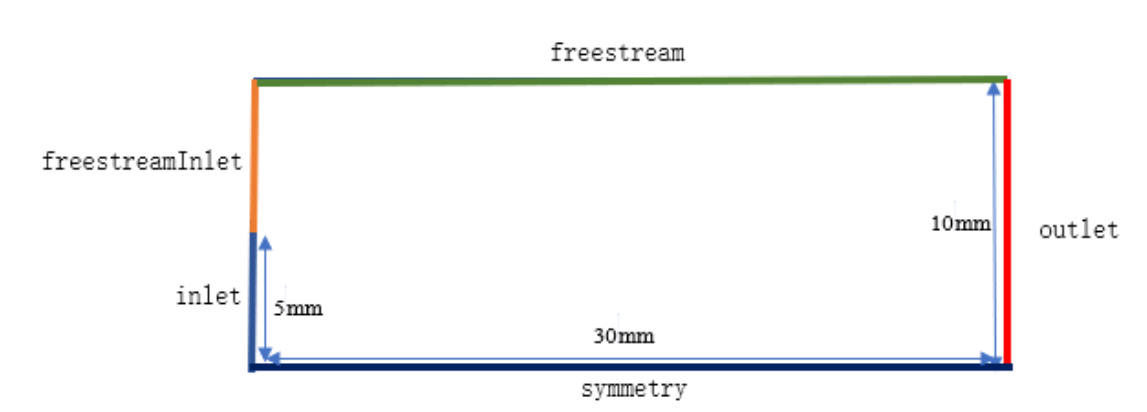
\includegraphics[width=\textwidth]{figs/geometry.png}
  \caption{Computational domain and boundary conditions for Ladenburg jet test case.}
  \label{fig:geometry}
\end{figure}

Since the case is axisymmetric, a wedge condition is applied to the front and back boundaries, as illustrated in Figure~\ref{fig:wedge}. The other boundaries are highlighted in color for context: the white boundary is the inlet, the green is the \texttt{freestreamInlet}, and the blue is the \texttt{freestream}.

\begin{figure}[H]
  \centering
  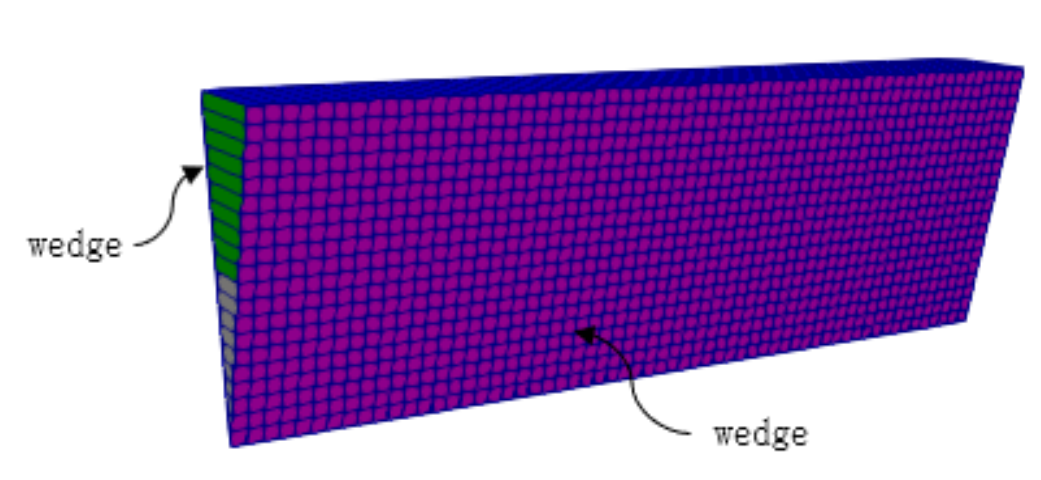
\includegraphics[width=\textwidth]{figs/wedge.png}
  \caption{Coarse grid ($g_0$) and wedge boundary conditions.}
  \label{fig:wedge}
\end{figure}

The domain is very tightly focused on the near-field region of the under-expanded jet since the purpose of the simulation is to correctly estimate the position of the Mach disc.

The folder \texttt{0} contains the fields $p$, $T$, and $U$ at a fairly well-converged state, as mentioned above. Converged solutions on coarser grids were interpolated on finer levels. In FLUENT only one simulation on the $g_2$ grid level was performed, as explained later on. The boundary conditions adopted in OpenFOAM and FLUENT are outlined in Table~\ref{tab:OF_BC} and Table 2, respectively.

The \texttt{waveTransmissive} condition applied at the outlet is used to limit the reflection of waves at boundaries such as outlets and inlets, which can be a problem with high Mach number flows. The \texttt{totalPressure} condition applied at the freestream boundary calculates pressure using one of four methods depending on the simulation case. In these highly compressible flows, a gamma value (the ratio of specific heats) is provided as part of the boundary condition, and since it is greater than 1, the pressure at the patch is given by"
%
\begin{equation}
  p_p = \frac{p_0}{(1 + 0.5 \psi G |U|^2)^{1/G}}
  \label{eq:total_pressure}
\end{equation}
%
for the total pressure $p_0$ and a coefficient $G = \frac{1 - \gamma}{\gamma}$. A similar boundary condition, \texttt{totalTemperature}, is also applied at the freestream boundary where the temperature at the patch, $T_p$, is given by:
%
\begin{equation}
  T_p = \frac{T_0}{1 + 0.5 \psi G |U|^2}
  \label{eq:total.temperature}
\end{equation}
%
The \texttt{noSlip} condition applied for velocity at the \texttt{freestreamInlet} is used here since this boundary represents the solid nozzle wall.

\begin{table}[H]
  \centering
  \caption{OpenFOAM boundary conditions for the Ladenburg jet case.}
  \label{tab:OF_BC}
  \begin{tabular}{ccccc} 
  \hline
    Boundary & p & T & U \\
    \hline
    inlet & fixedValue & fixedValue & fixedValue \\
    outlet & waveTransmissive & zeroGradient & inletOutlet \\
    freestream & totalPressure & totalTemperature & zeroGradient \\
    freestreamInlet & zeroGradient & fixedValue & noSlip \\
    \hline
  \end{tabular}
\end{table}

\begin{longtable}{>{\raggedright\arraybackslash}p{9cm}>{\raggedright\arraybackslash}p{5cm}}
%\caption{Boundary Conditions Table} \\
\caption{FLUENT boundary conditions for the Ladenburg jet case.} \\
 \hline
\textbf{Boundary Condition} & \textbf{Value or Specification} \\
\hline
\endfirsthead
%
\multicolumn{2}{c}%
{\tablename\ \thetable\ -- continued from previous page} \\
\hline
\textbf{Boundary Condition} & \textbf{Value or Specification} \\
\hline
\endhead
%
%\hline \multicolumn{2}{r}{Continued on next page} \\ \hline
\endfoot
%
\hline
\endlastfoot
%
\hline
%\multicolumn{2}{c}{\textbf{Boundary Conditions}} \\
%\hline
%
\textbf{Inlet} & \\
\hline
Velocity Specification Method & Reference Frame \\
Velocity Magnitude [m/s] & 315.6 \\
Supersonic/Initial Gauge Pressure [Pa] & \textbf{170675} \\
Temperature [K] & 247.1 \\
Outflow Gauge Pressure [Pa] & 0 \\
%Note: Reinjected particles do not change their injection association & \\
\hline
%
\textbf{Outlet} & \\
\hline
Backflow Reference Frame & Absolute \\
Gauge Pressure [Pa] & 0 \\
Pressure Profile Multiplier & 1 \\
Backflow Total Temperature [K] & 297 \\
Backflow Direction Specification Method & Normal to Boundary \\
%Note: Reinjected particles do not change their injection association & \\
Acoustic Wave Model & no \\
Backflow Pressure Specification & Total Pressure \\
Build artificial walls to prevent reverse flow? & Off \\
Radial Equilibrium Pressure Distribution & no \\
Average Pressure Specification? & no \\
Specify targeted mass flow rate & no \\
\hline
%
%\textbf{Outlet 2} & \\
%\hline
%Backflow Reference Frame & Absolute \\
%Gauge Pressure [Pa] & 0 \\
%Pressure Profile Multiplier & 1 \\
%Backflow Total Temperature [K] & 297 \\
%Backflow Direction Specification Method & Normal to Boundary \\
%%Note: Reinjected particles do not change their injection association & \\
%Acoustic Wave Model & no \\
%Backflow Pressure Specification & Total Pressure \\
%Build artificial walls to prevent reverse flow? & Off \\
%Radial Equilibrium Pressure Distribution & no \\
%Average Pressure Specification? & no \\
%Specify targeted mass flow rate & no \\
%\hline
%
\textbf{Symmetry} & \\
\hline
Type & wedge2 \\
Type & wedge1 \\
\hline
%
\textbf{Wall} & \\
\hline
Wall Thickness [m] & 0 \\
Heat Generation Rate [W/m$^3$] & 0 \\
Material Name & aluminum \\
Thermal BC Type & Temperature \\
Temperature [K] & 297 \\
Wall Motion & Stationary Wall \\
Shear Boundary Condition & No Slip \\
Convective Augmentation Factor & 1 \\
\hline
\end{longtable}

The numerical simulations were initialized with the initial conditions reported in Table~\ref{tab:OF_IC}:

\begin{table}[H]
  \centering
  \caption{OpenFOAM/FLUENT initial conditions for the Ladenburg jet case.}
  \label{tab:OF_IC}
  \begin{tabular}{cccc}
\hline
Boundary & Pressure (Pa) & Axial Velocity (m/s) & Temperature (K) \\
\hline
Inlet      & 271724 & 315.6 & 247.1 \\
Outlet     & 101325 & 0.0   &  - \\
Freestream & 101325 & 0.0   & 297 \\
\hline
\end{tabular}
\end{table}

In FLUENT a gauge pressure $p_{gauge}$ = 101326 Pa was imposed. Thus, the inlet pressure was given by the difference $p$ = $p_\infty$ - $p_{gauge}$ = 272000 - 101325 = 170675 Pa.

The \texttt{constant} directory contains the thermophysical and turbulence properties for the case. A \textbf{laminar} model is specified here in the turbulence file, and a \texttt{hePsiThermo} thermo type is used in the thermophysical file with a perfect gas equation of state and Sutherland viscosity model chosen. The choice of a laminar flow test cases was preferred as it avoid the additional level of complexity related to the assessment of the turbulence model's impact.

In the \texttt{system} directory, the \texttt{fvSchemes} file provides the flux scheme to be used by the solver to determine the upwinding used. The Kurganov and Tadmor schemes are the two options available, with the Kurganov chosen in this case:
%
\begin{verbatim}
interpolationSchemes
{
  default          linear;
  reconstruct(rho) vanLeer;
  reconstruct(U)   vanLeerV;
  reconstruct(T)   vanLeer;
}
\end{verbatim}
%
The \texttt{fvSolution} file with the case is short. The density-weighted variables, $\rho$, $\hat{U}$, and $\hat{E}$, are solved with a diagonal solver for the inviscid case, and the remaining parts of the Navier-Stokes equations are then included when $U$ and $e$ are solved by using a \texttt{smoothSolver}:
%
\begin{verbatim}
solvers
{
  "(rho|rhoU|rhoE)"
  {
    solver         diagonal;
  }
  U
  {
    solver         smoothSolver;
    smoother       GaussSeidel;
    nSweeps        2;
    tolerance      1e-10;
    relTol         0;
  }
  e
  {
    solver         smoothSolver;
    smoother       GaussSeidel;
    nSweeps        2;
    tolerance      1e-10;
    relTol         0;
  }
}
\end{verbatim}
%
The case is run by creating the mesh and running the application. The Mach number for the simulation could also be calculated as shown below in post-processing:
%
\begin{verbatim}
blockMesh
rhoCentralFoam
rhoCentralFoam -postProcess -func MachNo
\end{verbatim}

%%%%%%%%%%%%%%%%%%%%%%%%%%%%%%%%%%%%%%%%%%%%%%%%%%%
\section{Grid convergence}\label{sec:conv}
%%%%%%%%%%%%%%%%%%%%%%%%%%%%%%%%%%%%%%%%%%%%%%%%%%%
A simple grid convergence analysis was conducted in OpenFOAM to assess the sensitivity of key flow features to mesh resolution. Four mesh configurations were employed.
%- \textbf{Refined mesh}: 3.2 million hexahedral elements (25\% refinement from baseline)
%- \textbf{Baseline mesh}: 2.56 million hexahedral elements (as used in main simulations)
%- \textbf{Coarse mesh}: 1.72 million hexahedral elements (same as original Ladenburg experiment~\cite{Ladenburg})
The convergence criteria focused on critical parameters: Mach disk position and thickness, triple point location (radial and axial coordinates), velocity and pressure gradients across shock structures, density contour profiles in the jet shear layer.

Table~\ref{tab:grid_convergence} presents the quantitative comparison of key parameters across different mesh densities. All values show less than 3\% relative error variation between baseline and refined meshes, indicating converged solutions within acceptable engineering accuracy.

\begin{table}[H]
\centering
\caption{Grid convergence study results.}
\label{tab:grid_convergence}
\adjustbox{max width=\textwidth}{%
\begin{tabular}{lcccccc}
\hline
Parameter & Exp. & $g_0$ & $g_1$ & $g_2$ & $g_3$ & FLUENT\\
\hline
Mach disk axial position (mm) & 13.3 & 17.5 & 13.75 & 13.625 &  13.625 & \textbf{13.524} \\
Triple point radial position (mm) & 1.7 & 3.0 & 1.5 & 1.625 & 1.75 & \textbf{1.678} \\
%Peak Mach number & - & 2.15 & 2.17 & 2.18 & \\
%Density gradient magnitude ({$kg/m^4$}) & - & $4.2\times10^3$ & $4.5\times10^3$ & $4.6\times10^3$ & \\
\hline
\end{tabular}}
\end{table}

Figure~\ref{fig:conv} shows the distribution of density, pressure, temperature and velocity magnitude along the symmetry axis of the computational domain. Figure~\ref{fig:conv} visually demonstrates mesh independence in shock structure resolution already for the $g_2$ level which was thus adopted as baseline also in FLUENT. The refined mesh shows improved resolution of the barrel shock curvature without significant changes to the overall flow topology.
%
\begin{figure}[H]
    \centering
   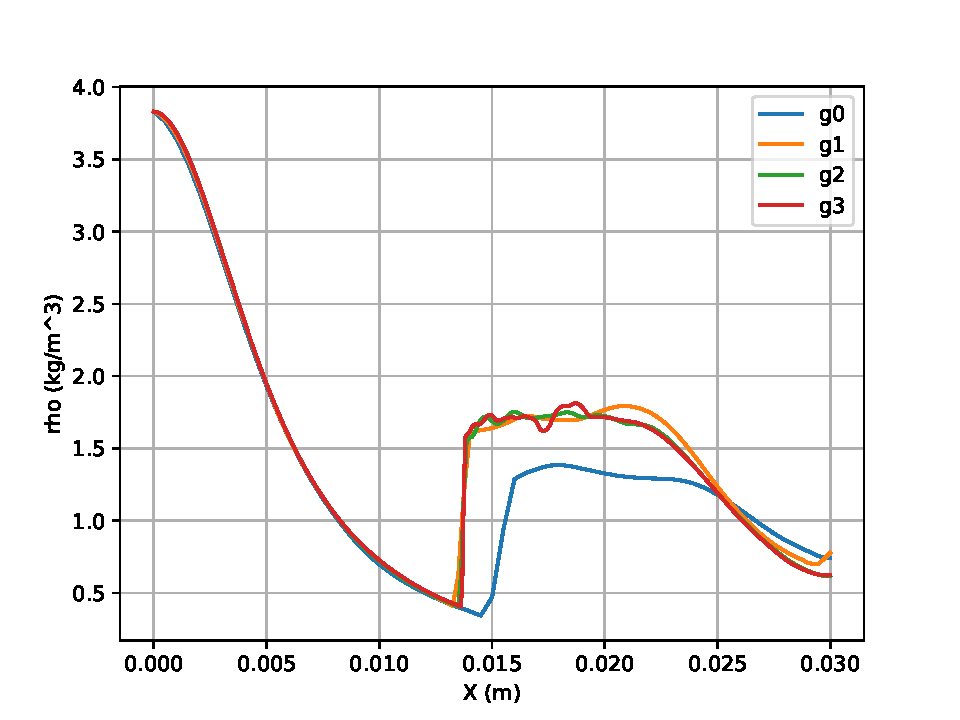
\includegraphics[width=0.495\textwidth]{figs/rho.pdf}
   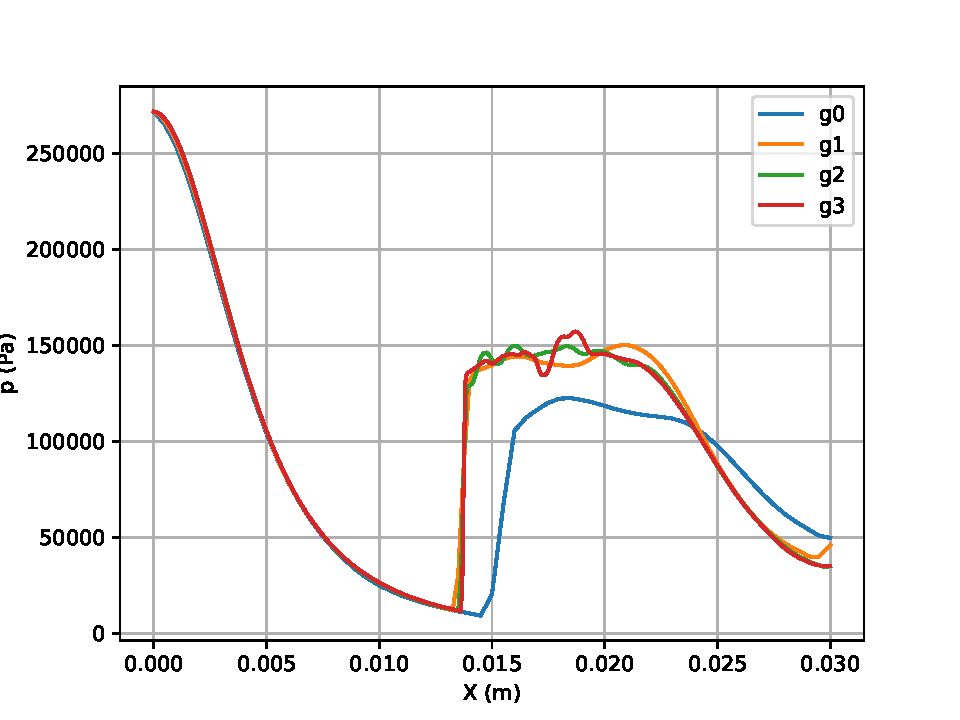
\includegraphics[width=0.495\textwidth]{figs/pres.pdf}\\
   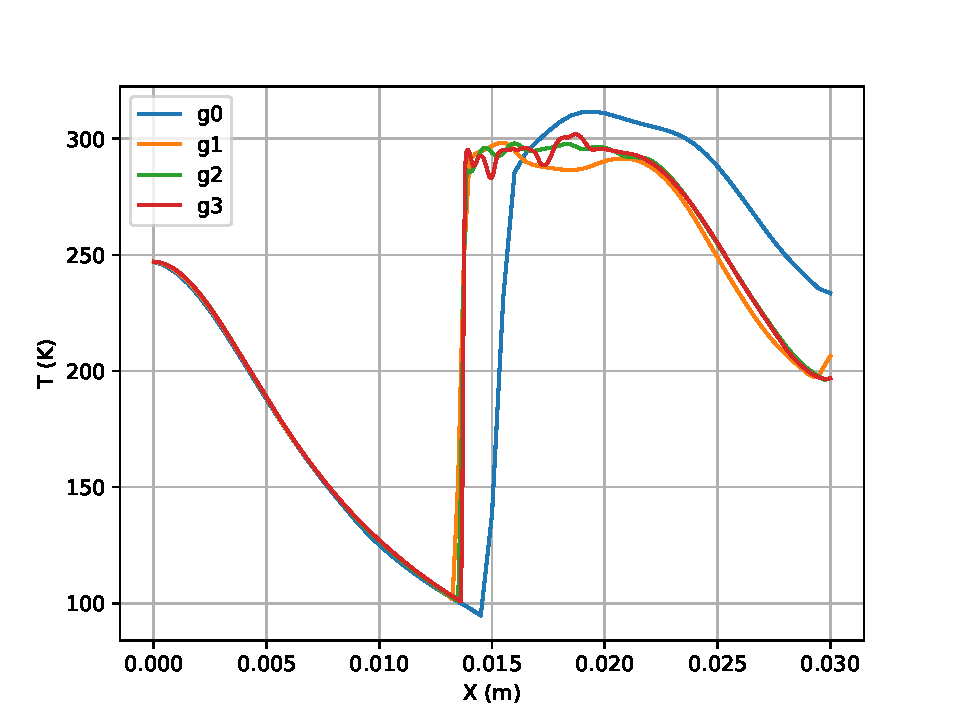
\includegraphics[width=0.495\textwidth]{figs/temp.pdf}
   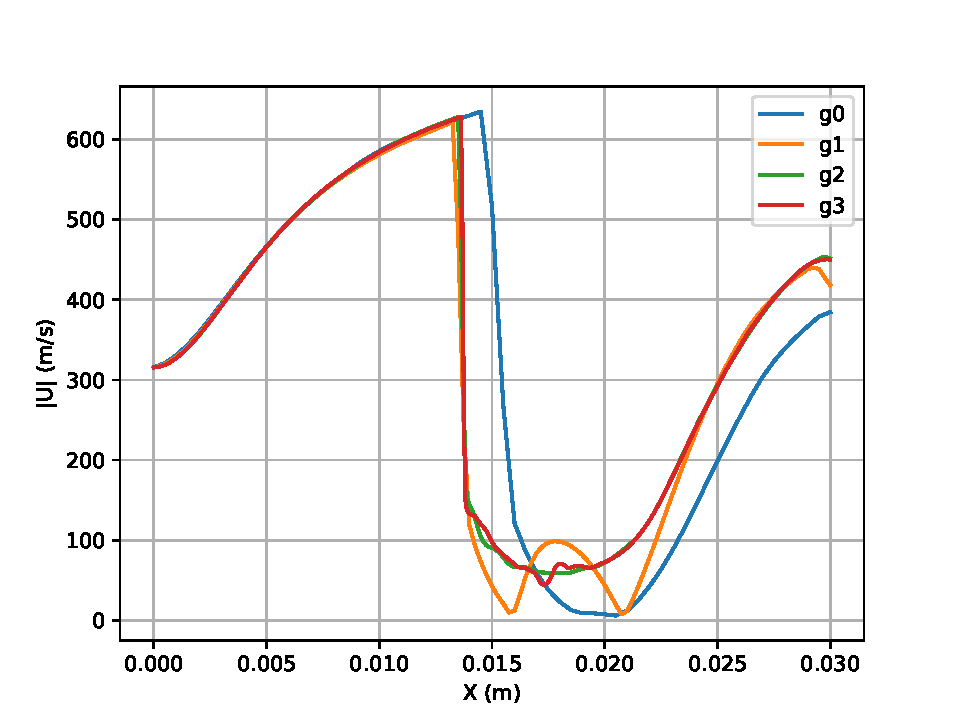
\includegraphics[width=0.495\textwidth]{figs/vel.pdf}
    \caption{Distribution of density, pressure, temperature and velocity magnitude along the symmetry axis of the computational domain used for the grid convergence analysis performed in OpenFOAM on four levels.}
    \label{fig:conv}
\end{figure}

%\newpage 

%%%%%%%%%%%%%%%%%%%%%%%%%%%%%%%%%%%%
\section{Results}\label{sec:results}
%%%%%%%%%%%%%%%%%%%%%%%%%%%%%%%%%%%%
This section presents the results of the simulation of the Ladenburg jet test case. Numerical solution obtained by OpenFOAM and FLUENT were compared with experimental data from~\cite{ladenburg1949interferometric}. Figures~\ref{fig:OFplots}, \ref{fig:OFPimpleplots} and \ref{fig:Fplots} show density, pressure, temperature and velocity magnitude contour plots obtained by OpenFOAM and FLUENT, respectively, on the $g_2$ grid level. Even if the different colorbar style, slightly masks similarities and differences, a satisfactory qualitative agreement between the solvers' solutions was achieved.

It is generally acknowledged that \texttt{rhoPimpleFoam} \textit{is not a really compressible solver} by admitting that \textit{only density-based solver is a real compressible solver}, like that Roe method or HLL method, and any other kind of approximate Riemann solver. In this regard, \texttt{rhoCentralFoam} is a \textit{real compressible solver} which employs central scheme. 

Even if \texttt{rhoPimpleFoam} is a highly validated solve, it is a pressure-based solver instead of a density-based solver. It does not have the entropy fix, thus, when dealing with hyperbolic set of equations, \texttt{rhoPimpleFoam} it should be expected to perform worse than \texttt{rhoCentralFoam}. On the other hand, \texttt{rhoCentralFoam} should do a better job at capturing shocks and other discontinuities, even if not with high resolution due to the additional dissipation introduced by the fix. This aspect, indeed, is clearly visible in Figure~\ref{fig:OFplots} and \ref{fig:OFPimpleplots}  where the unsteady nature of the test case is clearly visible in the \texttt{rhoPimpleFoam} solutions while fluctuations are typically more strongly smeared out in the \texttt{rhoCentralFoam} solutions and the shock location is more accurately predicted.

The code in Listings~\ref{lst:pproc}-\ref{lst:FLUENT_vs_EXP_stack} were used to post-process all numerical results, transforming (flipping, padding, rotating) and vertically stacked raw images.

Figure~\ref{fig:rho_OF_vs_FLUENT} compares the density field obtained by OpenFOAM and FLUENT on the $g_2$ grid level. A good agreement in the representation of the fluid dynamic topological structures was achieved. The location of the Mach stem is similar while some differences can be observed at the outlet, due to the different treatment of the non-reflective BC implemented by the solvers. Some reverse flow can indeed can be noted in FLUENT solution as well as a more accurate resolution of the shock front downstream, thanks to a III order MUSCL scheme adopted in the last iterations.

Figures~\ref{fig:prof_rho}-\ref{fig:prof_V} show the profile of density, pressure, temperature and velocity magnitude along the symmetry axis of the computational domain. 
Several, if not all, compressible OpenFOAM solvers are compared to have an idea about how they perform. Few observations can be made. The \texttt{rhoCentralFoam} and \texttt{rhoPimpleCentralFoam} solvers perform best. The \texttt{sonicFoam} appears to be most dissipative. The OpenFOAM \texttt{rhoPimpleFoam} solver predicts a shock position further downstream and manifests a more oscillatory behaviour.

Figures~\ref{fig:rho_OF_vs_EXP_viridis} and \ref{fig:rho_FLUENT_vs_EXP_viridis} compare the density field computed, respectively, by OpenFOAM and FLUENT with the experimental results while Figure~\ref{fig:rho_OF_vs_FLUENT_viridis} compare the density field computed by the two solvers. The position of the Mach stem presents some differences with FLUENT solution closer to the experimental values. This is probably due to the slightly different BCs applied by the two solvers. Further fine tuning in OpenFOAM may improve the agreement. This behaviour was also observed in other numerical results, presented in Figures~\ref{fig:comp1}-\ref{fig:comp3}. In general, the density isocontour lines show a good agreement between the solutions computed by the two solvers, as well as with the experimental results, especially upstream of the shock structure.

\begin{figure}[H]
  \centering
  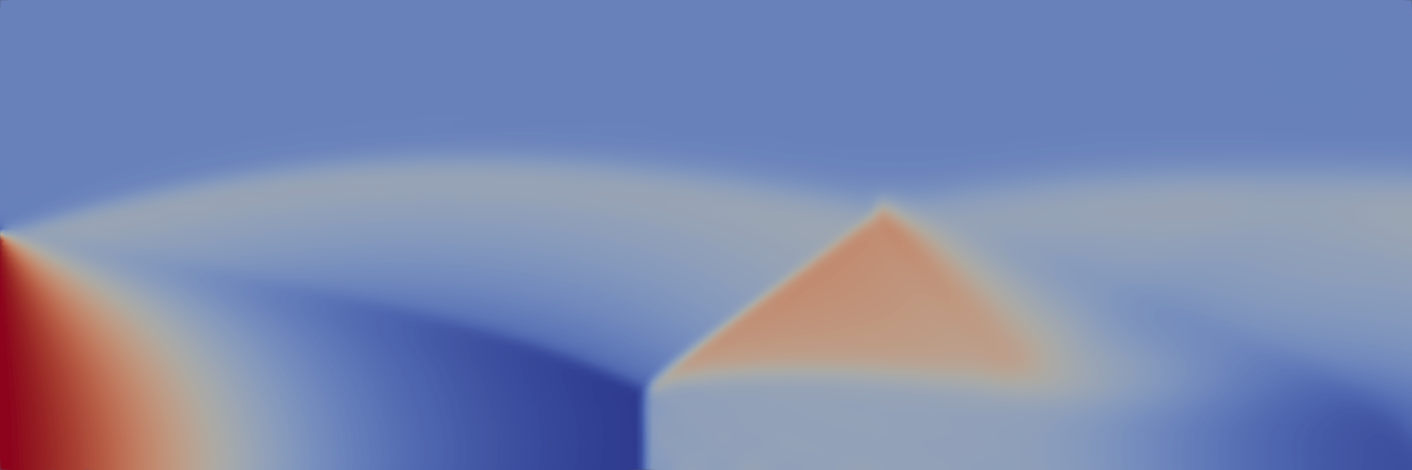
\includegraphics[width=0.495\textwidth]{figs/rho.png}
  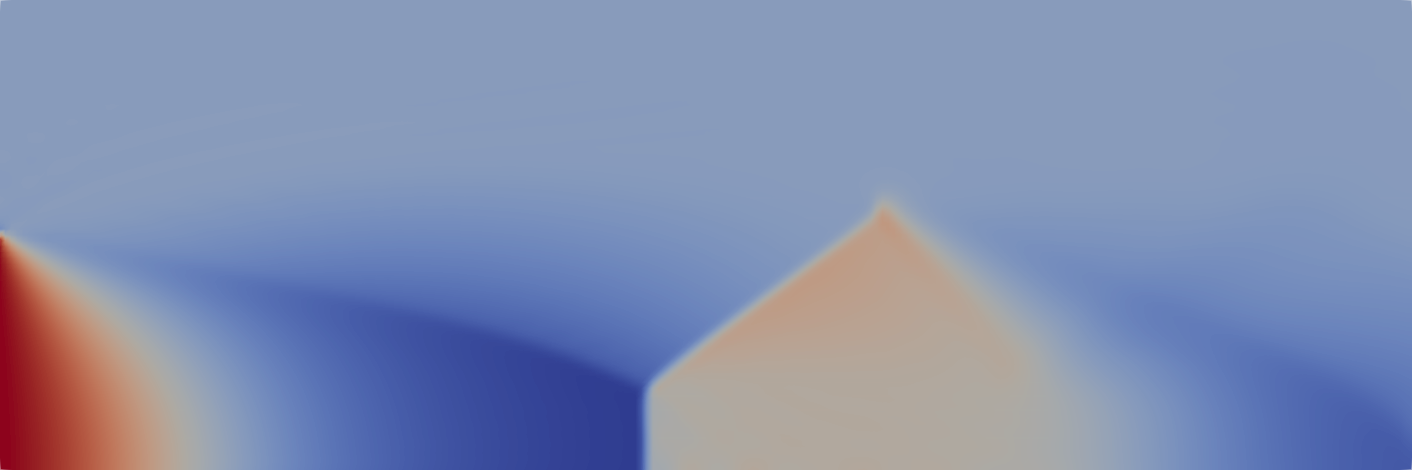
\includegraphics[width=0.495\textwidth]{figs/p.png}\\
  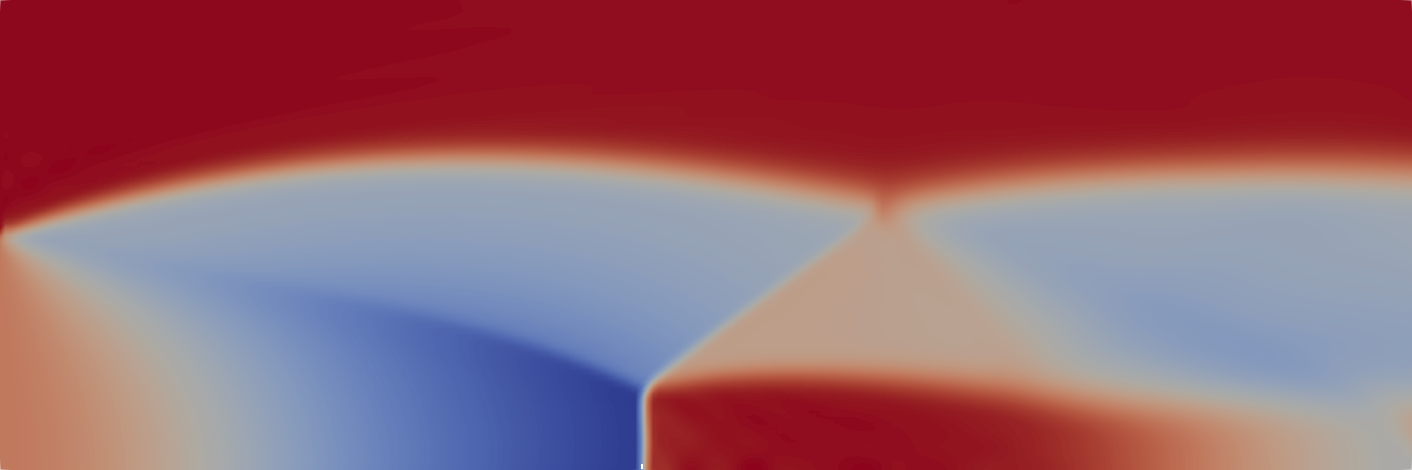
\includegraphics[width=0.495\textwidth]{figs/T.png}
  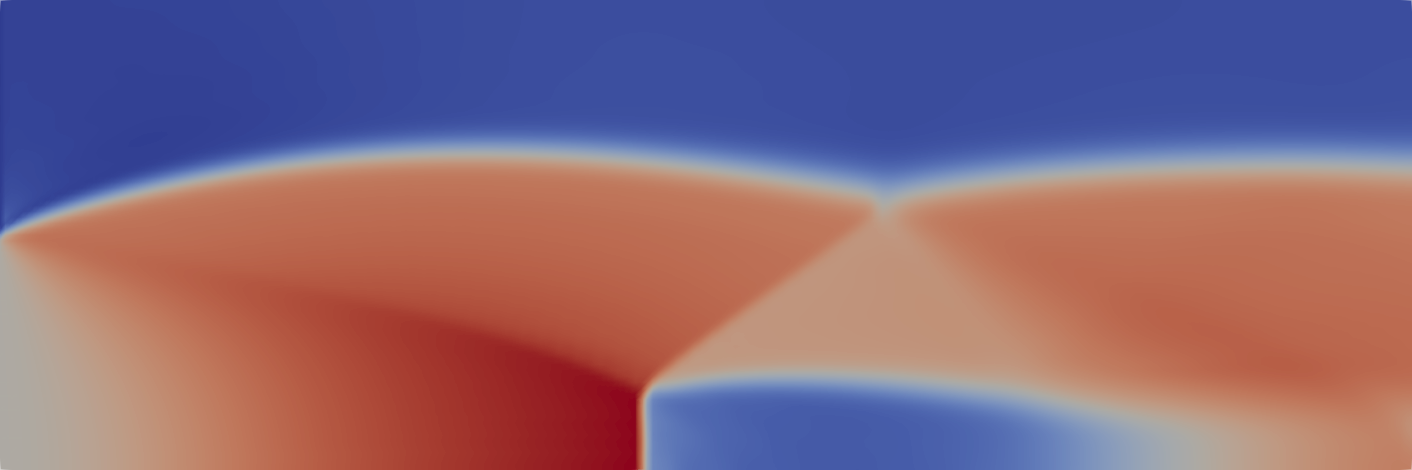
\includegraphics[width=0.495\textwidth]{figs/U.png}
  \caption{Density, pressure, temperature and velocity magnitude contour plots for the Ladenburg jet case obtained by OpenFOAM \texttt{rhoCentralFOAM} solver on the $g_2$ grid level.}
  \label{fig:OFplots}
\end{figure}

\begin{figure}[H]
  \centering
  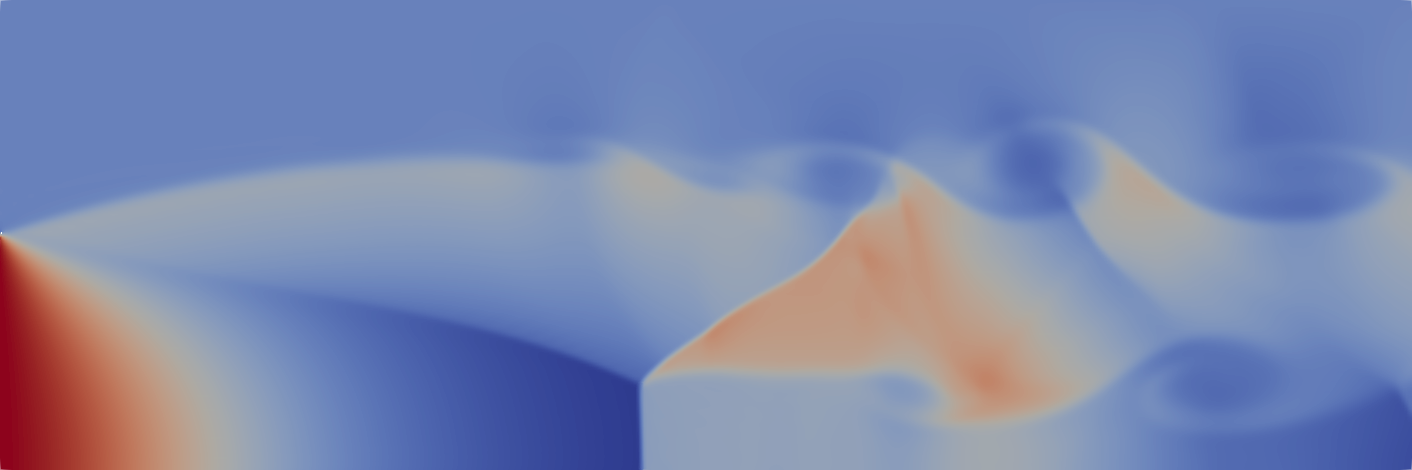
\includegraphics[width=0.495\textwidth]{figs/g3/rho.png}
  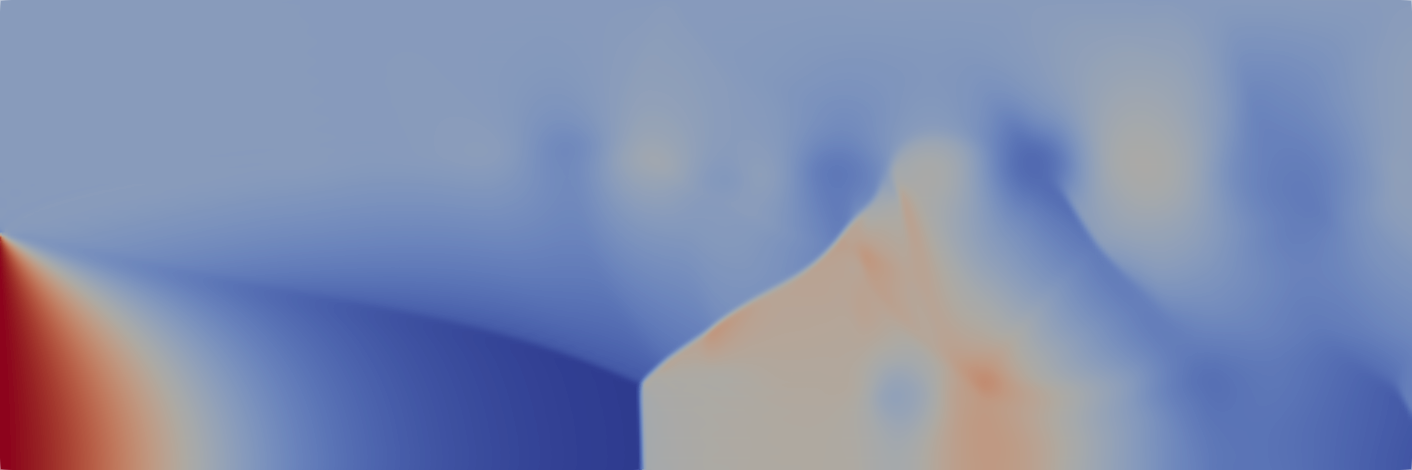
\includegraphics[width=0.495\textwidth]{figs/g3/p.png}\\
  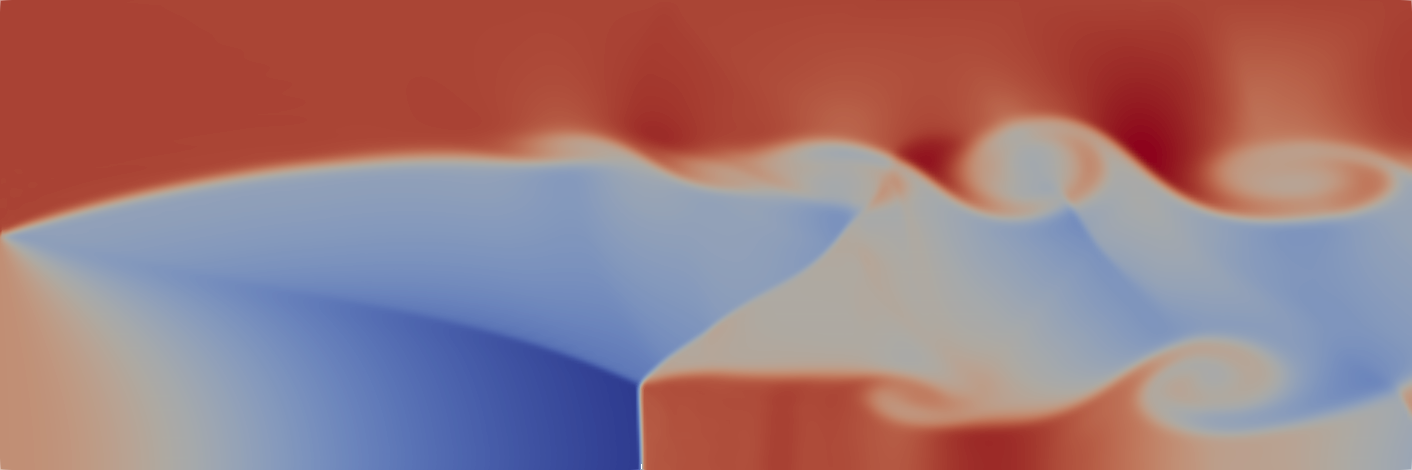
\includegraphics[width=0.495\textwidth]{figs/g3/T.png}
  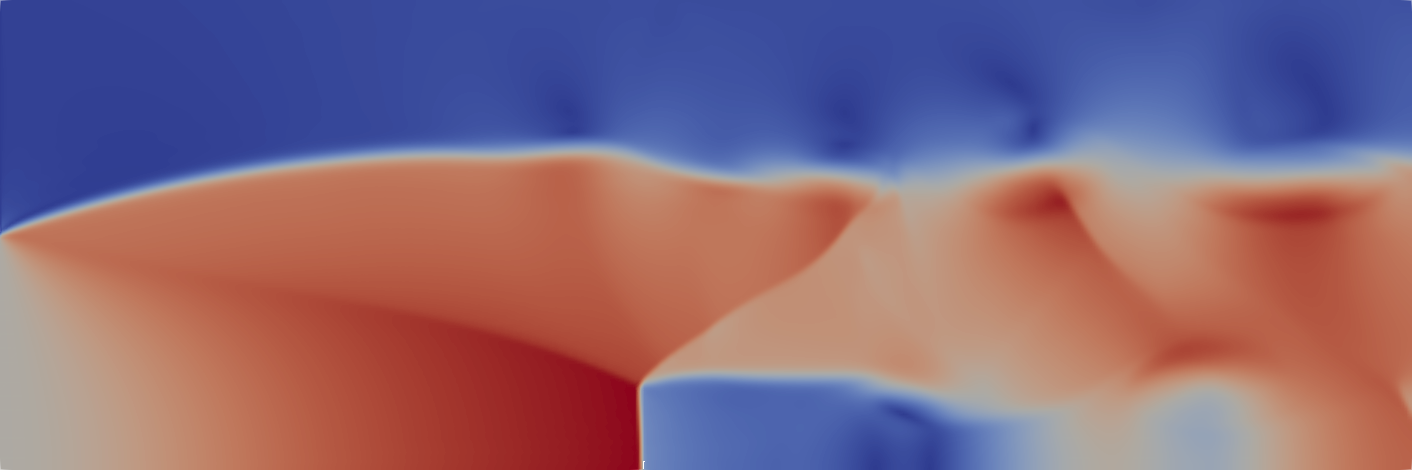
\includegraphics[width=0.495\textwidth]{figs/g3/U.png}
  \caption{Density, pressure, temperature and velocity magnitude contour plots for the Ladenburg jet case obtained by OpenFOAM \texttt{rhoCentralFOAM} solver on the $g_3$ grid level.}
  \label{fig:OFg3plots}
\end{figure}

\begin{figure}[H]
  \centering
  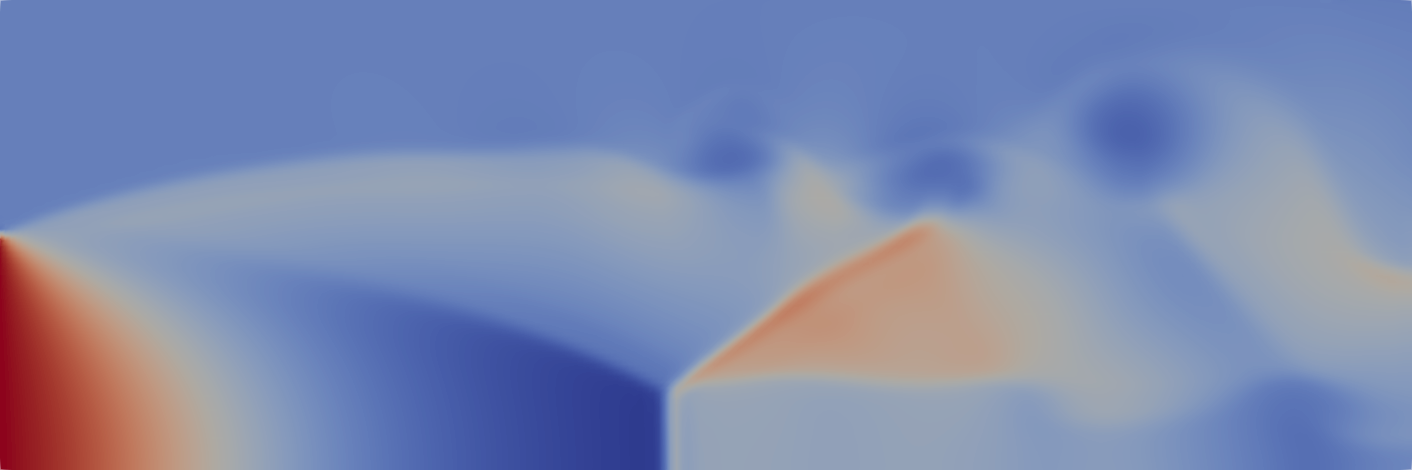
\includegraphics[width=0.495\textwidth]{figs/rhoPimpleFoam/rho.png}
  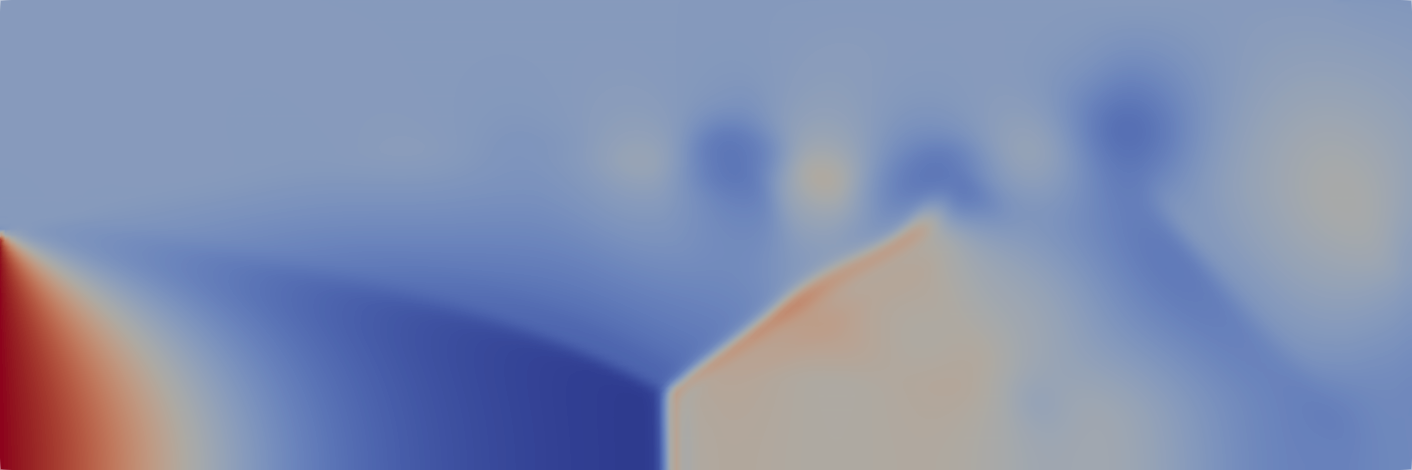
\includegraphics[width=0.495\textwidth]{figs/rhoPimpleFoam/p.png}\\
  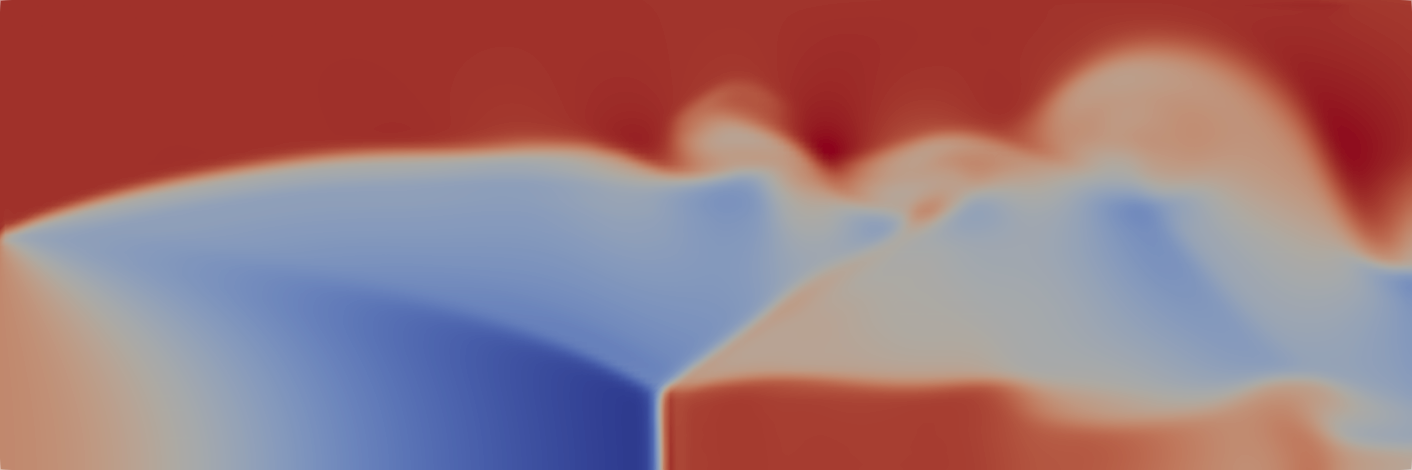
\includegraphics[width=0.495\textwidth]{figs/rhoPimpleFoam/T.png}
  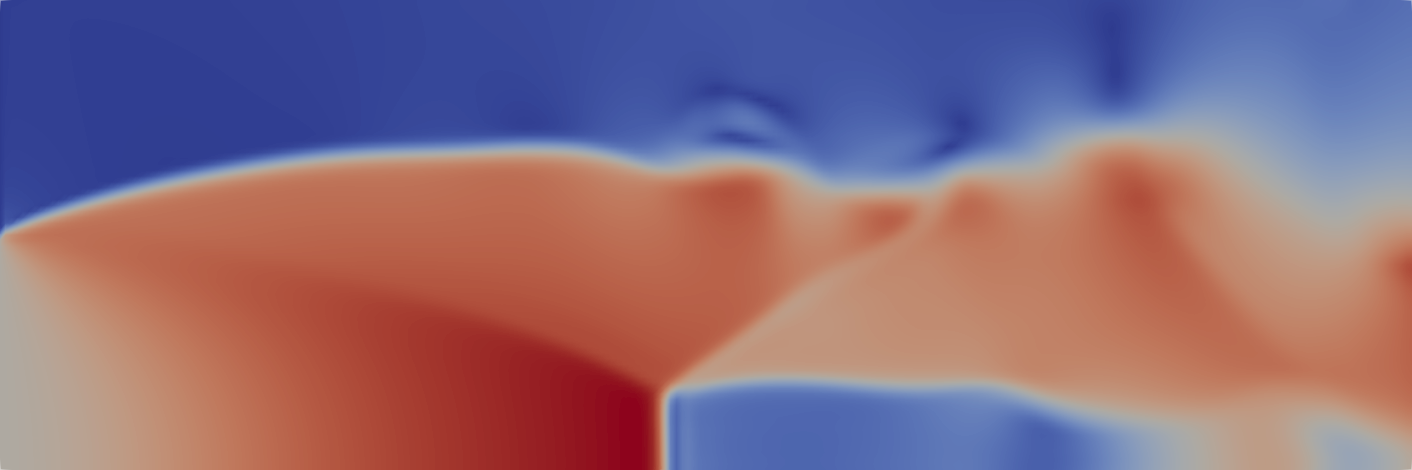
\includegraphics[width=0.495\textwidth]{figs/rhoPimpleFoam/U.png}
  \caption{Density, pressure, temperature and velocity magnitude contour plots for the Ladenburg jet case obtained by OpenFOAM \texttt{rhoPimpleFOAM} solver on the $g_2$ grid level.}
  \label{fig:OFPimpleplots}
\end{figure}

\begin{figure}[H]
  \centering
  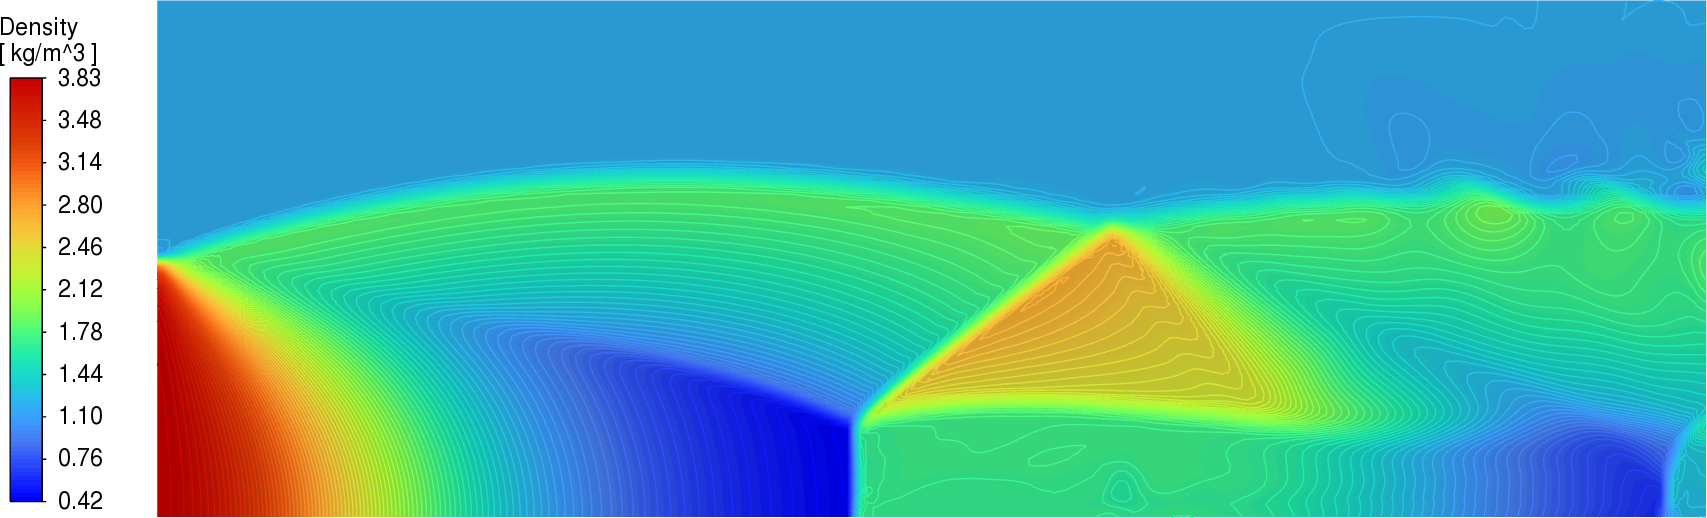
\includegraphics[width=0.495\textwidth]{figs/fluent_rho2.png}
  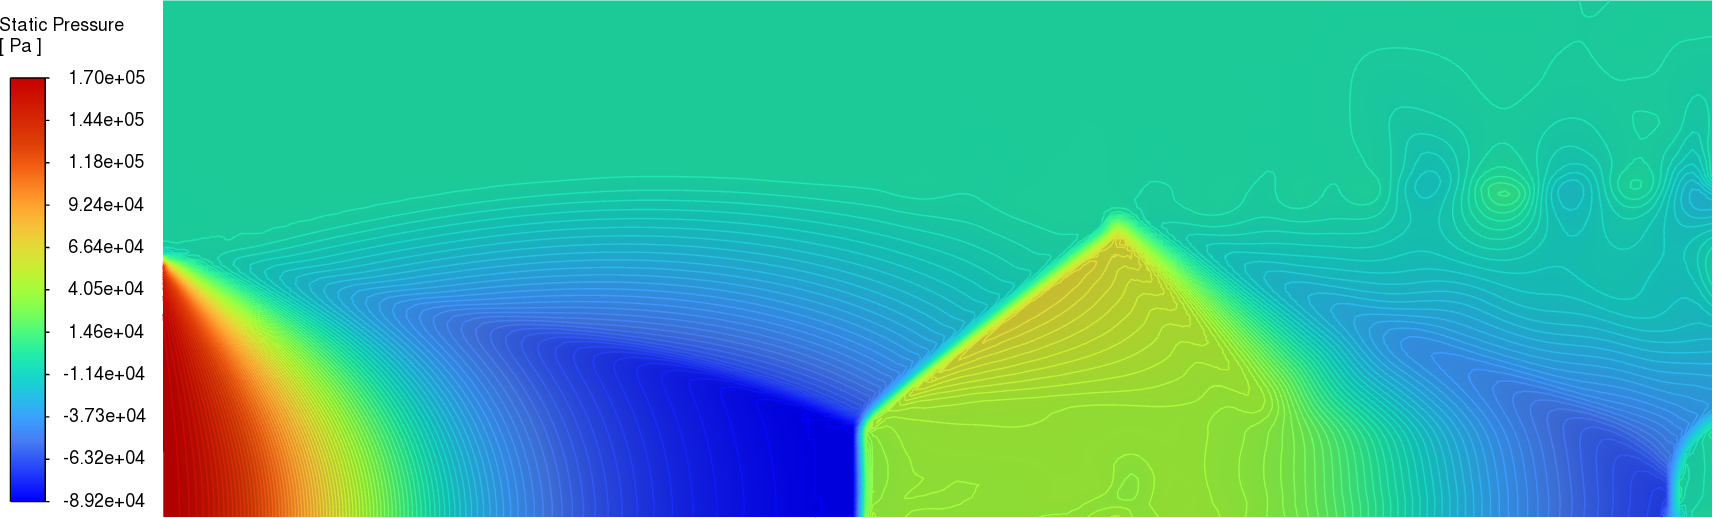
\includegraphics[width=0.495\textwidth]{figs/fluent_p2.png}\\
  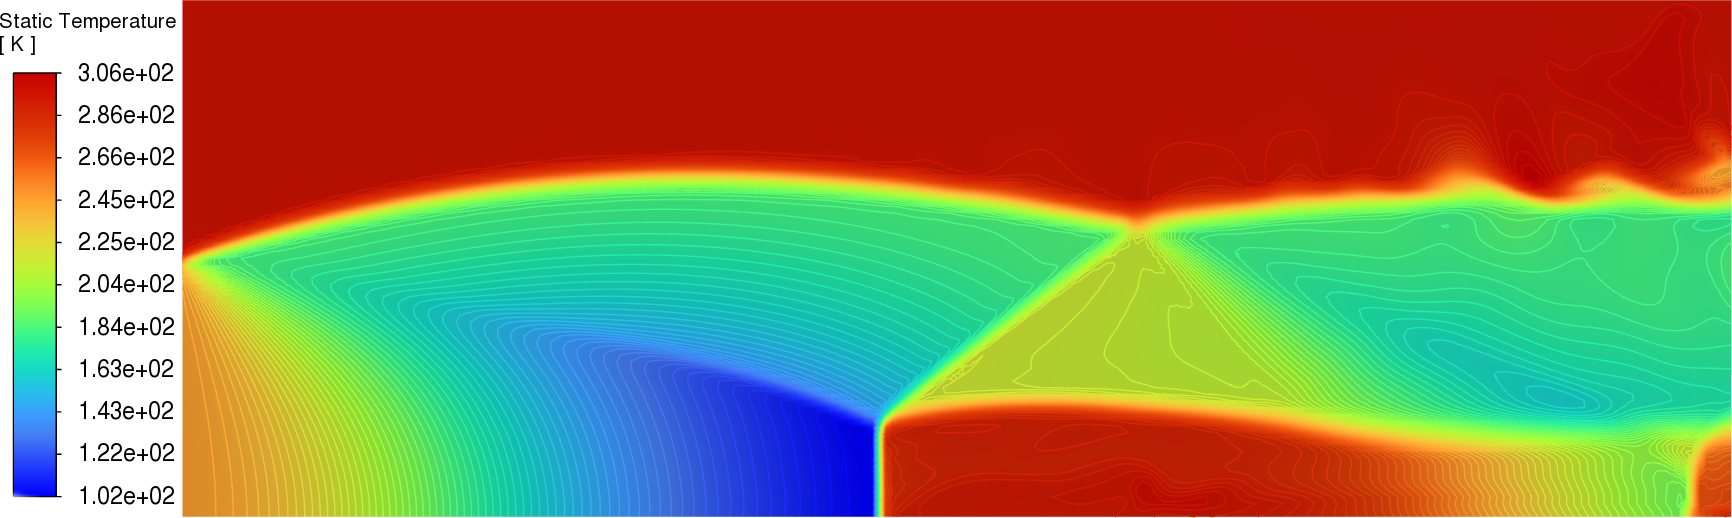
\includegraphics[width=0.495\textwidth]{figs/fluent_T2.png}
  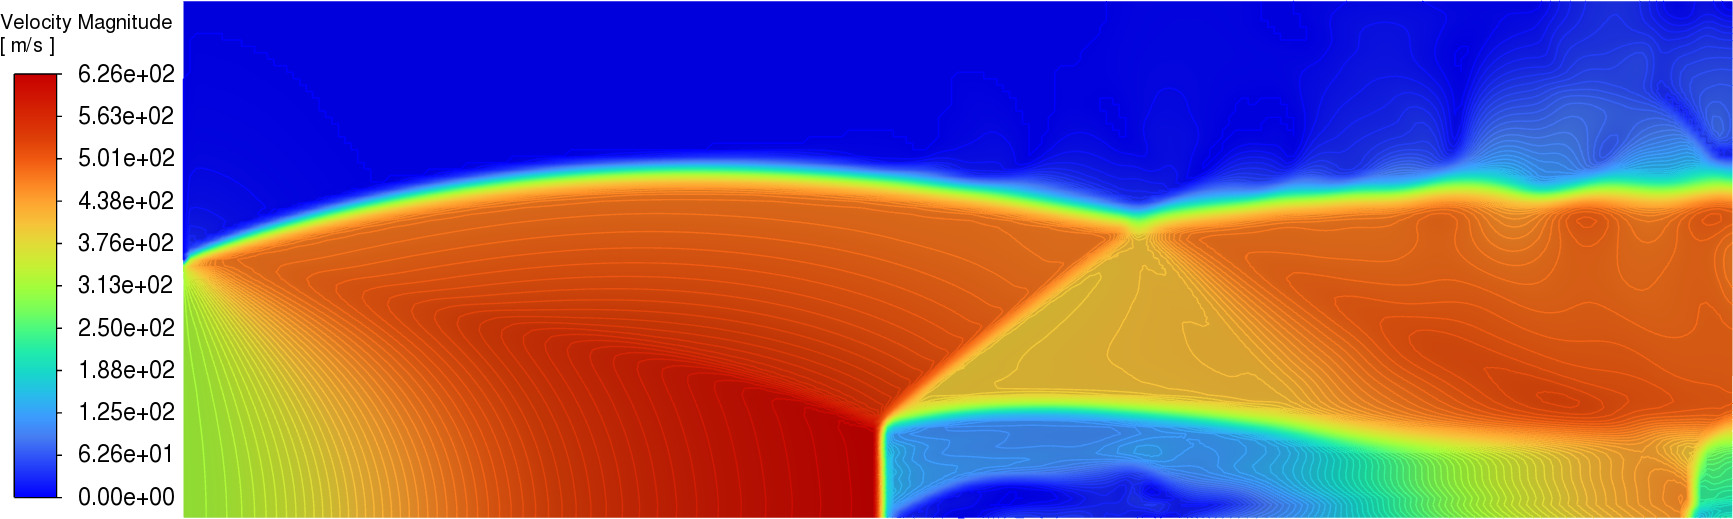
\includegraphics[width=0.495\textwidth]{figs/fluent_v2.png}
  \caption{Density, pressure, temperature and velocity magnitude contour plots for the Ladenburg jet case obtained by FLUENT on the $g_2$ grid level.}
  \label{fig:Fplots}
\end{figure}

\begin{lstlisting}[language=Python, caption=Post-processing functions script., label=lst:pproc]
import cv2
import numpy as np
import matplotlib.pyplot as plt

def ensure_3_channels(img):
    """Converts RGBA to RGB if needed."""
    if img.shape[2] == 4:
        return cv2.cvtColor(img, cv2.COLOR_BGRA2BGR)
    return img

def pad_image(img, top=0, bottom=0, left=0, right=0, color=(255, 255, 255)):
    """Adds padding to image on all sides."""
    return cv2.copyMakeBorder(img, top, bottom, left, right, cv2.BORDER_CONSTANT, value=color)

def rotate_image(img, angle):
    """
    Rotates image by a given angle (90, 180, 270).
    
    Args:
        img (np.array): Input image.
        angle (int): Must be 90, 180, or 270.
    Returns:
        np.array: Rotated image.
    """
    if angle == 90:
        return cv2.rotate(img, cv2.ROTATE_90_CLOCKWISE)
    elif angle == 180:
        return cv2.rotate(img, cv2.ROTATE_180)
    elif angle == 270:
        return cv2.rotate(img, cv2.ROTATE_90_COUNTERCLOCKWISE)
    else:
        print(f"Invalid rotation angle: {angle}. Supported angles: 90, 180, 270.")
        return img

def flip_image(img, direction='horizontal'):
    """
    Flips image either horizontally or vertically.

    Args:
        img (np.array): Input image.
        direction (str): 'horizontal' or 'vertical'
    Returns:
        np.array: Flipped image.
    """
    if direction == 'horizontal':
        return cv2.flip(img, 1)
    elif direction == 'vertical':
        return cv2.flip(img, 0)
    else:
        print(f"Invalid flip direction: {direction}. Use 'horizontal' or 'vertical'.")
        return img

def create_spacer(width, height, color=(255, 255, 255)):
    """Creates a solid-color spacer image."""
    spacer = np.zeros((height, width, 3), dtype=np.uint8)
    spacer[:] = color
    return spacer

def stack_images_vertically_with_padding_rotation_flipping(
    image_paths,
    output_path,
    image_options=None,
    spacing=0,
    spacing_color=(255, 255, 255)
):
    """
    Stacks images vertically with custom padding, rotation, flipping, and spacing.

    Args:
        image_paths (list): List of paths to input images.
        output_path (str): Path to save stacked image.
        image_options (list): List of dicts with parameters for each image:
            - 'pad': dict like {'top': 10, 'bottom': 20, ...}
            - 'rotate': int (90, 180, 270)
            - 'flip': str ('horizontal', 'vertical')
        spacing (int): Number of pixels between images.
        spacing_color (tuple): Color of spacing line.
    """
    images = []

    for i, path in enumerate(image_paths):
        img = cv2.imread(path, cv2.IMREAD_UNCHANGED)
        img = ensure_3_channels(img)

        # Apply transformations if provided
        opts = image_options[i] if image_options and i < len(image_options) else {}

        # Flip
        if "flip" in opts:
            img = flip_image(img, opts["flip"])

        # Rotate
        if "rotate" in opts:
            img = rotate_image(img, opts["rotate"])

        # Pad
        pad = opts.get("pad", {})
        top = pad.get("top", 0)
        bottom = pad.get("bottom", 0)
        left = pad.get("left", 0)
        right = pad.get("right", 0)
        pad_color = pad.get("color", (255, 255, 255))
        img = pad_image(img, top, bottom, left, right, pad_color)

        images.append(img)

    # Resize all images to match first image's width
    target_width = images[0].shape[1]
    resized_images = []
    for img in images:
        h, w = img.shape[:2]
        scale = target_width / w
        new_size = (target_width, int(h * scale))
        resized_img = cv2.resize(img, new_size)
        resized_images.append(resized_img)

    # Add spacing between images
    if spacing > 0:
        spacer = create_spacer(target_width, spacing, spacing_color)
        spaced_images = []
        for i, img in enumerate(resized_images):
            spaced_images.append(img)
            if i < len(resized_images) - 1:
                spaced_images.append(spacer)
        final_images = spaced_images
    else:
        final_images = resized_images

    # Stack them vertically
    stacked = np.vstack(final_images)

    # Save result
    cv2.imwrite(output_path, stacked)
    print(f"Saved stacked image to: {output_path}")

def plot_stacked_image(image_path):
    img = plt.imread(image_path)
    plt.figure(figsize=(8, 12))
    plt.imshow(cv2.cvtColor(img, cv2.COLOR_BGR2RGB))
    plt.axis("off")
    plt.tight_layout(pad=0)
    plt.show()
\end{lstlisting}

\begin{lstlisting}[language=Python, caption=Script to stack and plot numerical results of OpenFOAM and FLUENT., label=lst:stacking]
# Define paths to input images
image_paths = [ "../SIMS/g2/rho.png",     # OpenFOAM simulation output
                "../DATA/fluent/Frho.png" # ANSYS Fluent simulation output
]

image_transformations = [
    # OpenFOAM image settings
    {   "pad": {"top": 0, "bottom": 0, "left": 0, "right": 0}, 
        "rotate": 0 
    },
    # ANSYS Fluent image settings
    {   "pad": {"top": 0, "bottom": 0, "left": 0, "right": 0}, 
        "rotate": 180, "flip": "horizontal" 
    }
]

stack_images_vertically_with_padding_rotation_flipping(
    image_paths=image_paths,
    output_path="stacked_rho_OF_vs_FLUENT.png",
    image_options=image_transformations,
    spacing=1,
    spacing_color=(0, 0, 0) # black space
)

plot_stacked_image("stacked_rho_OF_vs_FLUENT.png")
\end{lstlisting}

\begin{figure}[H]
    \centering
    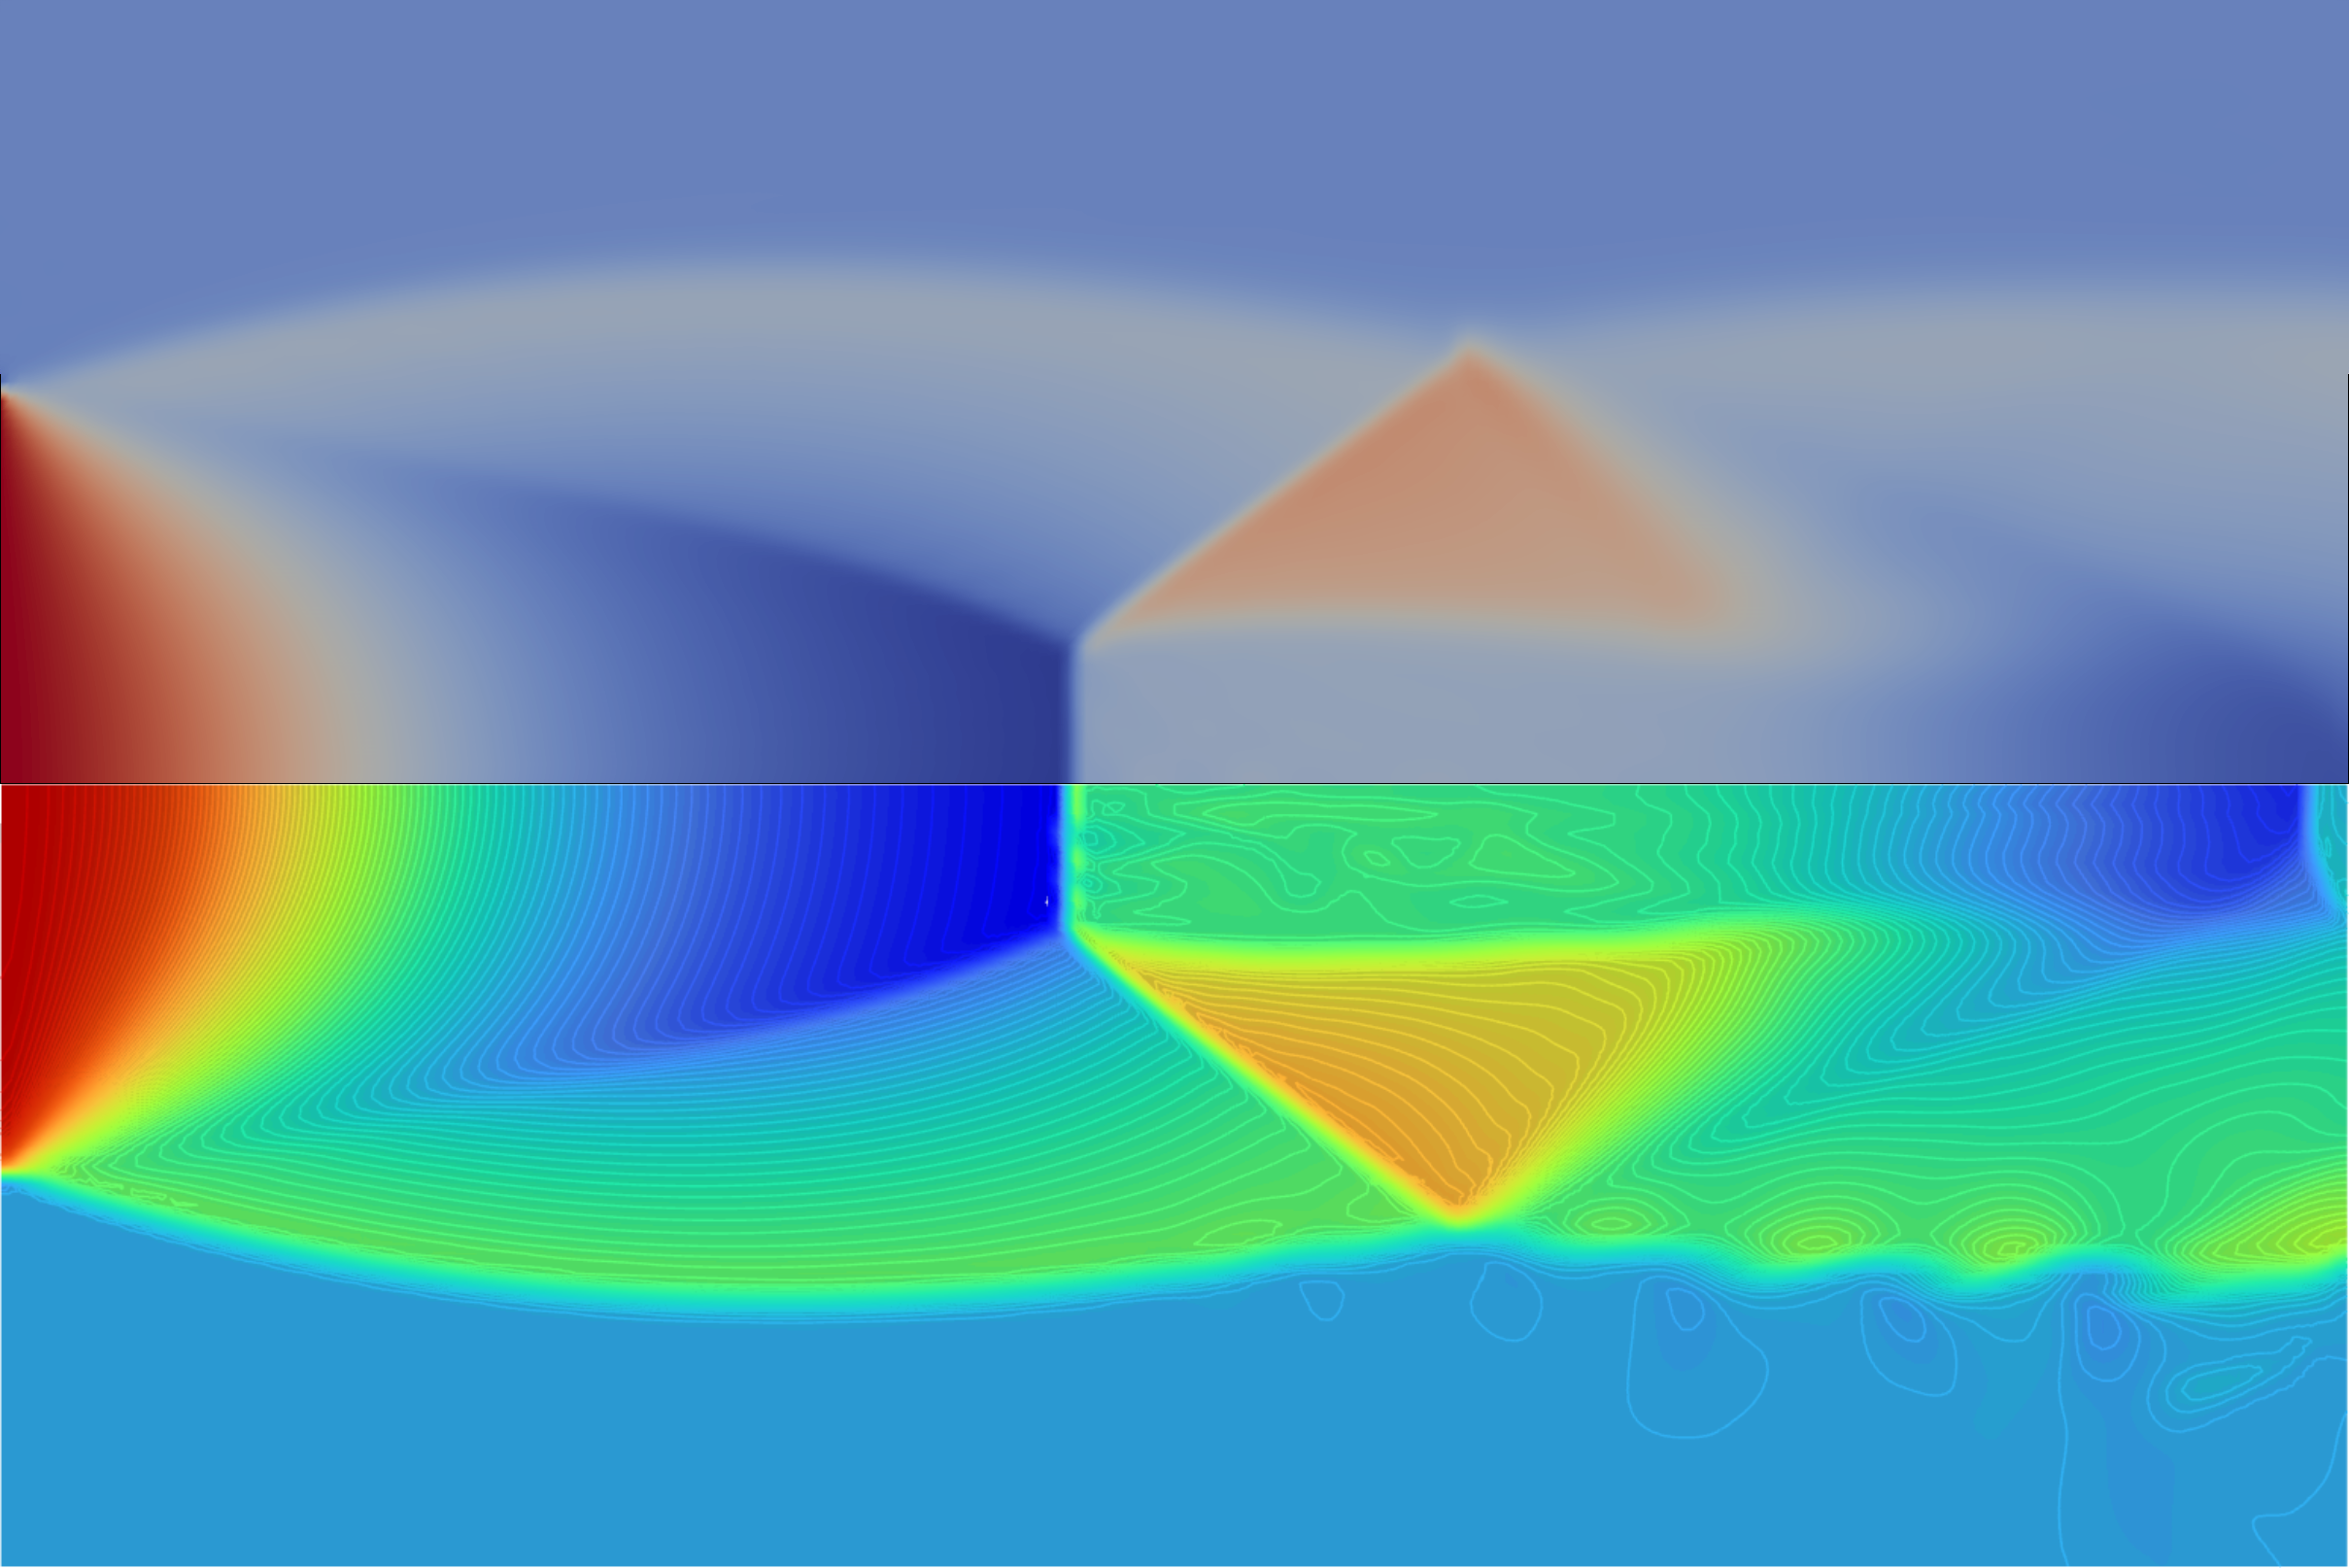
\includegraphics[width=0.925\linewidth]{figs/stacked_rho_OF_vs_FLUENT.png}
    \caption{Density contour of the supersonic jet computed by OpenFOAM \texttt{rhoCentralFoam} on the $g_2$ grid level (upper panel) and FLUENT (lower panel). The values of the density contours are provided in $kg/m^3$.}
    \label{fig:rho_OF_vs_FLUENT}
\end{figure}

\begin{figure}[H]
    \centering
    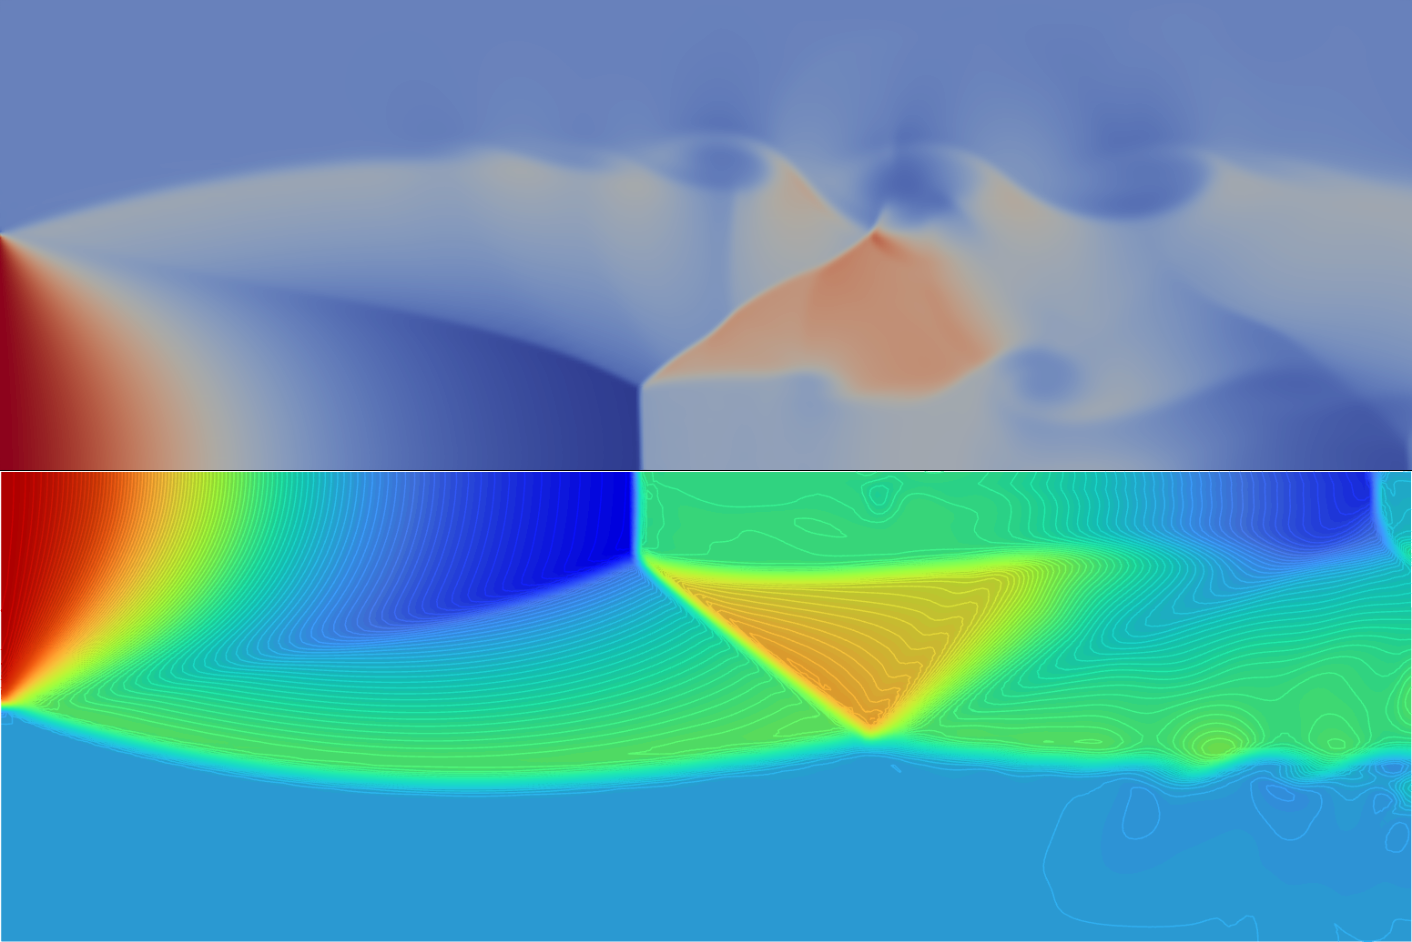
\includegraphics[width=0.925\linewidth]{figs/stacked_rho_OFg3_vs_FLUENT.png}
    \caption{Density contour of the supersonic jet computed by OpenFOAM \texttt{rhoCentralFoam} on the $g_3$ grid level (upper panel) and FLUENT (lower panel). The values of the density contours are provided in $kg/m^3$.}
    \label{fig:rho_OFg3_vs_FLUENT}
\end{figure}

\begin{figure}[H]
    \centering
    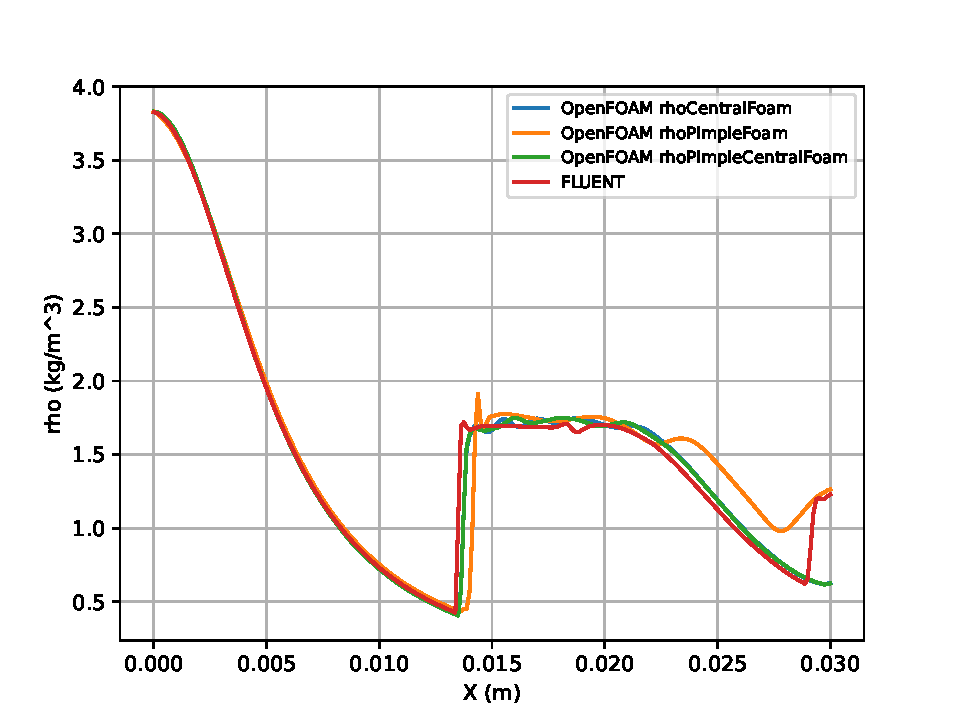
\includegraphics[width=0.9\linewidth]{figs/profile_density_OF_vs_F.pdf}
    \caption{Axial density profile obtained by OpenFOAM and FLUENT on the $g_2$ grid.}
    \label{fig:prof_rho}
\end{figure}
\begin{figure}[H]
    \centering
    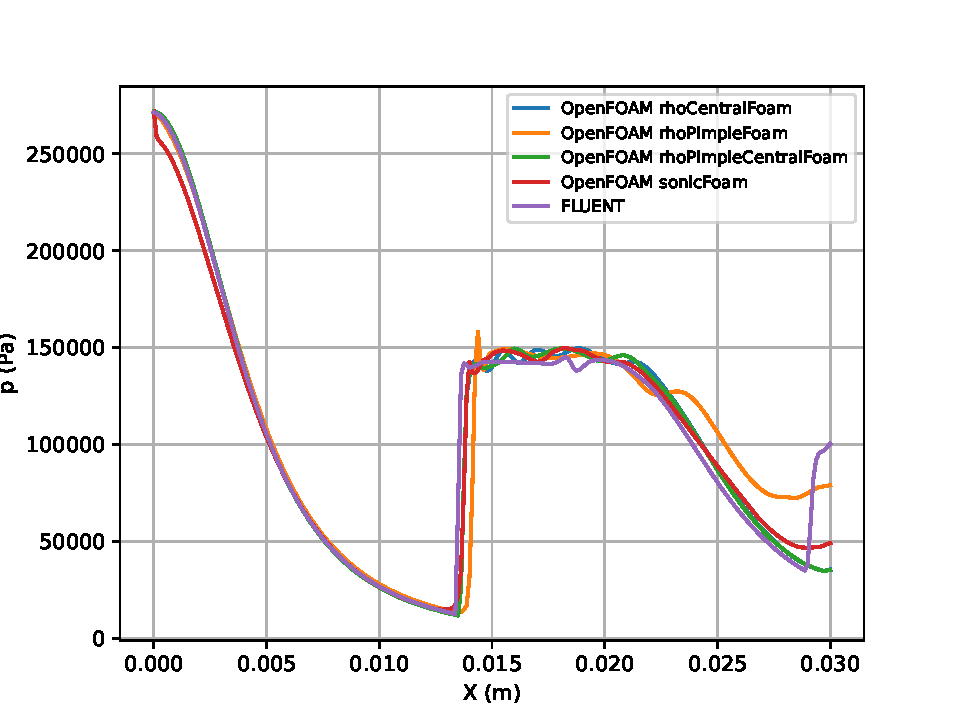
\includegraphics[width=0.9\linewidth]{figs/profile_pressure_OF_vs_F.pdf}
    \caption{Axial pressure profile obtained by OpenFOAM and FLUENT on the $g_2$ grid.}
    \label{fig:prof_p}
\end{figure}
\begin{figure}[H]
    \centering
    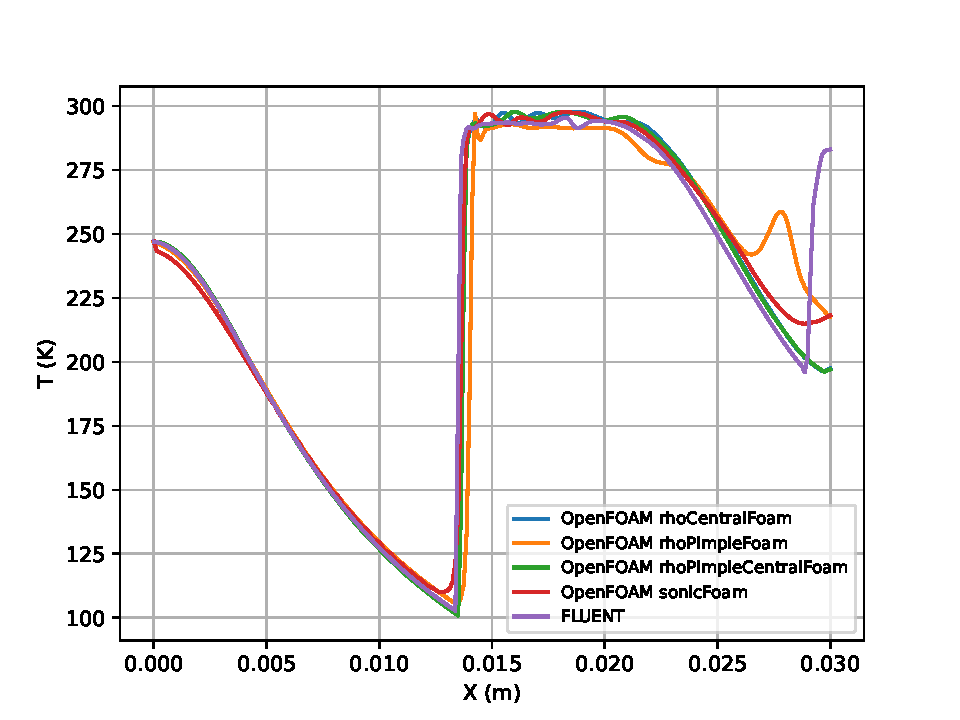
\includegraphics[width=0.9\linewidth]{figs/profile_temperature_OF_vs_F.pdf}
    \caption{Axial temperature profile obtained by OpenFOAM and FLUENT on the $g_2$ grid.}
    \label{fig:prof_T}
\end{figure}
\begin{figure}[H]
    \centering
    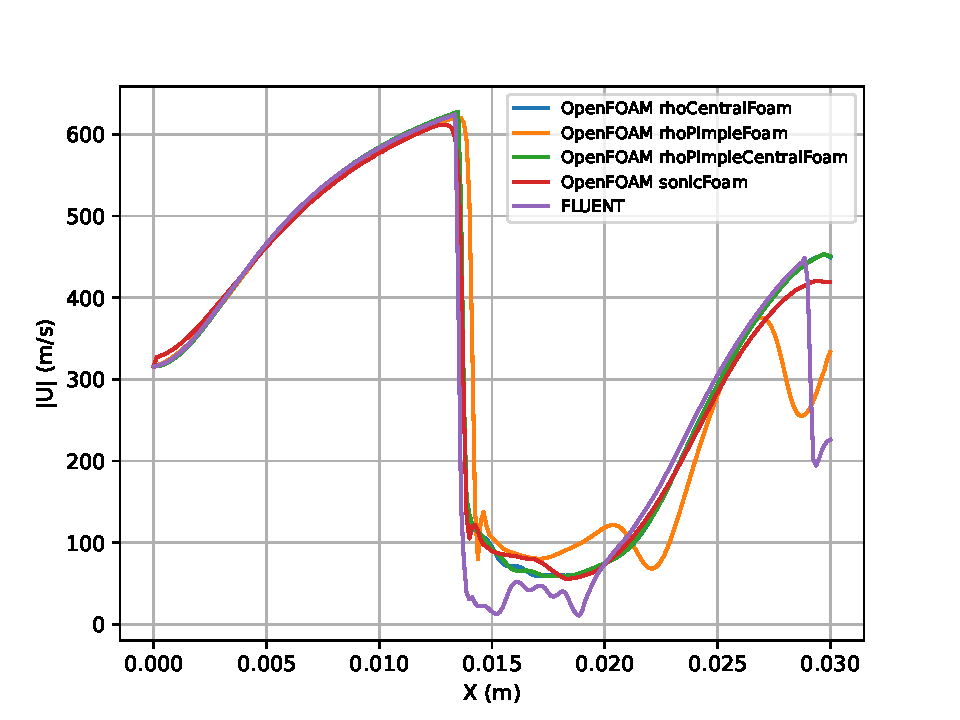
\includegraphics[width=0.9\linewidth]{figs/profile_velocity_mag_OF_vs_F.pdf}
    \caption{Axial velocity profile obtained by OpenFOAM and FLUENT on the $g_2$ grid.}
    \label{fig:prof_V}
\end{figure}

\begin{figure}[H]
    \centering
    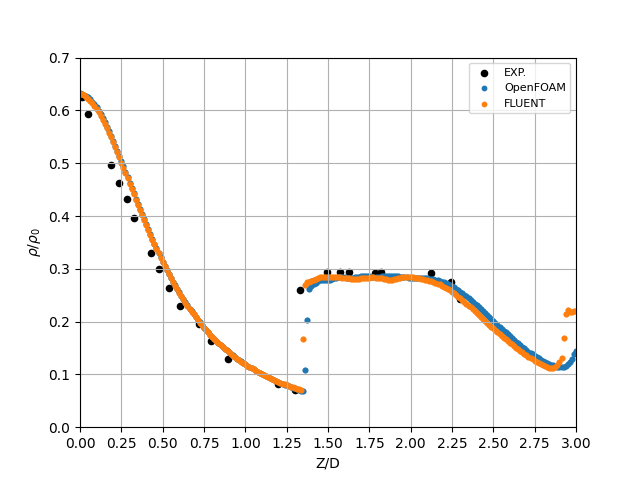
\includegraphics[width=0.85\linewidth]{figs/rho_ratio_vs_ZoD.png}
    \caption{The ratio $\rho$/$\rho_0$ (density at fixed distance R from axis for various jets/tank density) as a function of the ratio Z/D (distance from orifice/orifice diameter) for R/D=0.1.}
    \label{fig:density_ratio}
\end{figure}

\begin{figure}[H]
    \centering
    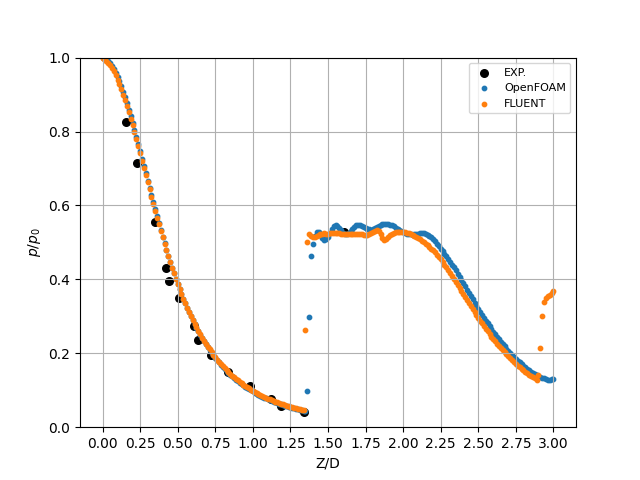
\includegraphics[width=0.85\linewidth]{figs/pressure_ratio_vs_ZoD.png}
    \caption{The ratio $p$/$p_0$ (pressure at fixed distance R from axis for various jets/tank density) as a function of the ratio Z/D (distance from orifice/orifice diameter) for R/D=0.0.}
    \label{fig:pressure_ratio}
\end{figure}

\begin{lstlisting}[language=Python, caption=Script to post-process results of OpenFOAM and experimental data., label=OF_vs_EXP_stack]
image_paths = [ "../SIMS/g2/rho_cut.png",  # OpenFOAM simulation results
                "../DATA/greenshields.png" # Exp. by Greenshields et al.
]

image_transformations = [
  { "pad": {"top": 0, "bottom": 0, "left": 40, "right": 15}, "rotate": 0 },
  { "pad": {"top": 0, "bottom": 0, "left": 0, "right": 0}, "rotate": 0 }
]

stack_images_vertically_with_padding_rotation_flipping(
    image_paths=image_paths,
    output_path="stacked_rho_OF_vs_EXP.png",
    image_options=image_transformations,
    spacing=1,
    spacing_color=(0, 0, 0) # black space
)

plot_stacked_image("stacked_rho_OF_vs_EXP.png")
\end{lstlisting}

\begin{figure}[H]
    \centering
    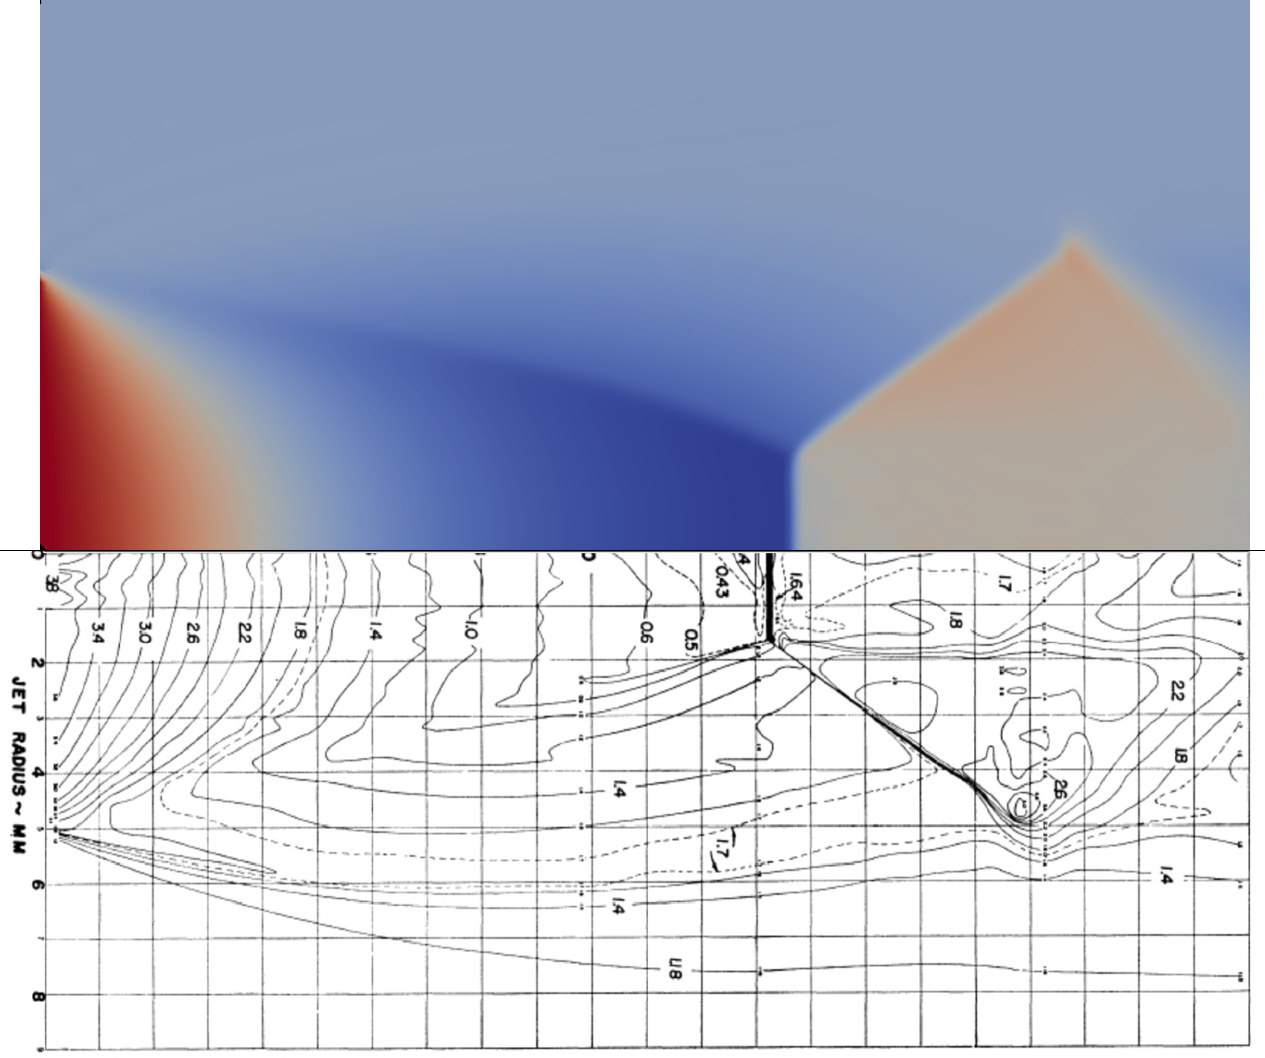
\includegraphics[width=0.95\linewidth]{figs/stacked_rho_OF_vs_EXP.png}
    \caption{Density distribution of the supersonic jet measured by Ladenburg~\cite{ladenburg1949interferometric} (lower of panel), and computational results (upper panel) obtained with OpenFOAM. The values of the density contours are provided in $kg/m^3$.}
    \label{fig:rho_OF_vs_EXP}
\end{figure}

\begin{lstlisting}[language=Python, caption=Script to stack and plot numerical results of FLUENT and experimental data., label=lst:FLUENT_vs_EXP_stack]
image_paths = [ "../DATA/fluent/Frho_cut.png", # Fluent simulation results
                "../DATA/greenshields.png" # Exp. by Greenshields et al.
]

image_transformations = [
  { "pad": {"top": 0, "bottom": 0, "left": 35, "right": 15}, "rotate": 0 }
  { "pad": {"top": 0, "bottom": 0, "left": 0, "right": 0},  "rotate": 0 }
]

stack_images_vertically_with_padding_rotation_flipping(
    image_paths=image_paths,
    output_path="stacked_rho_FLUENT_vs_EXP.png",
    image_options=image_transformations,
    spacing=1,
    spacing_color=(0, 0, 0) # black space
)

plot_stacked_image("stacked_rho_FLUENT_vs_EXP.png")
\end{lstlisting}

%\begin{figure}[H]
%    \centering
%    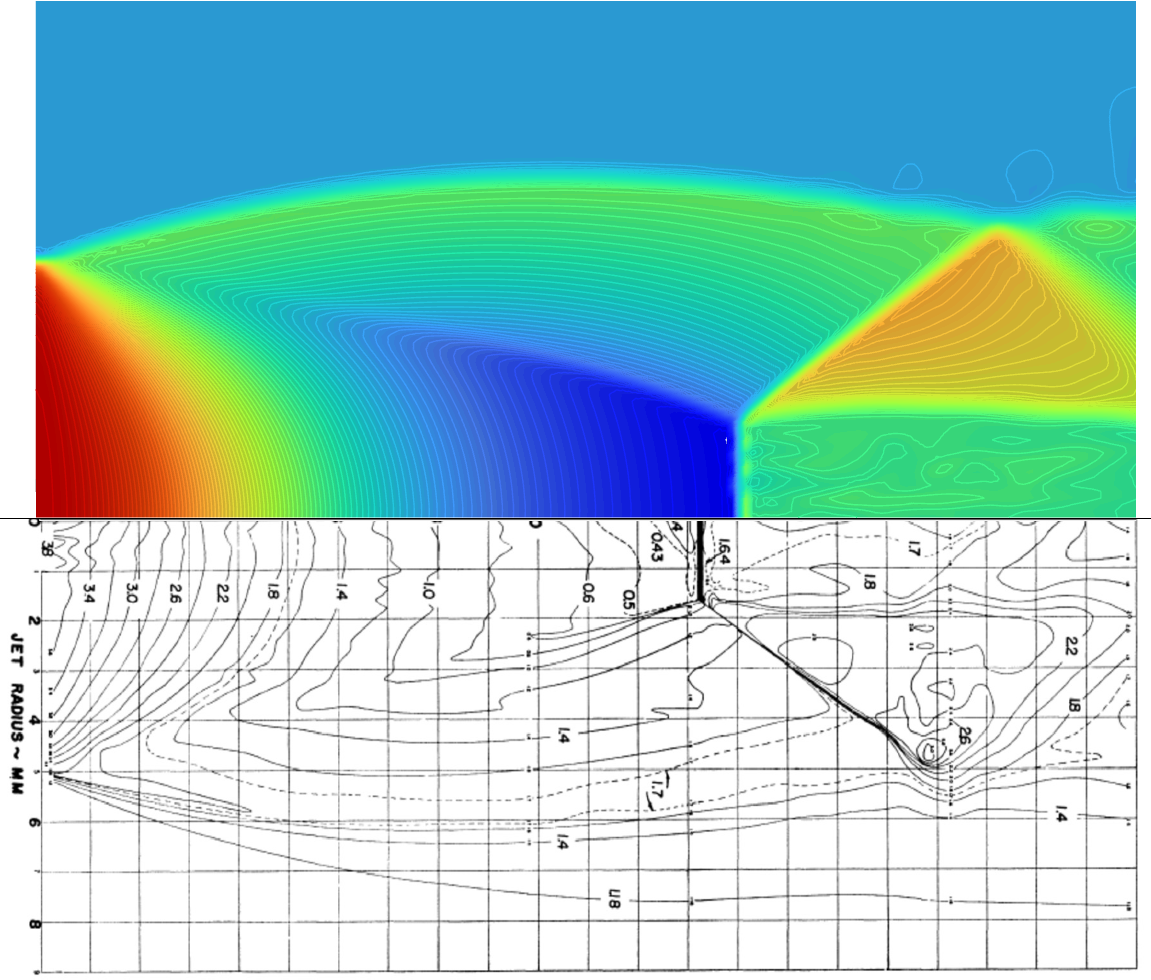
\includegraphics[width=0.95\linewidth]{figs/stacked_rho_FLUENT_vs_EXP.png}
%    \caption{Density distribution of the supersonic jet measured by %Ladenburg~\cite{ladenburg1949interferometric} (lower of panel), and computational %results (upper panel) obtained with FLUENT. The values of the density contours are %provided in $kg/m^3$.}
%    \label{fig:rho_FLUENT_vs_EXP}
%\end{figure}

%NEW
\begin{figure}[H]
    \centering
    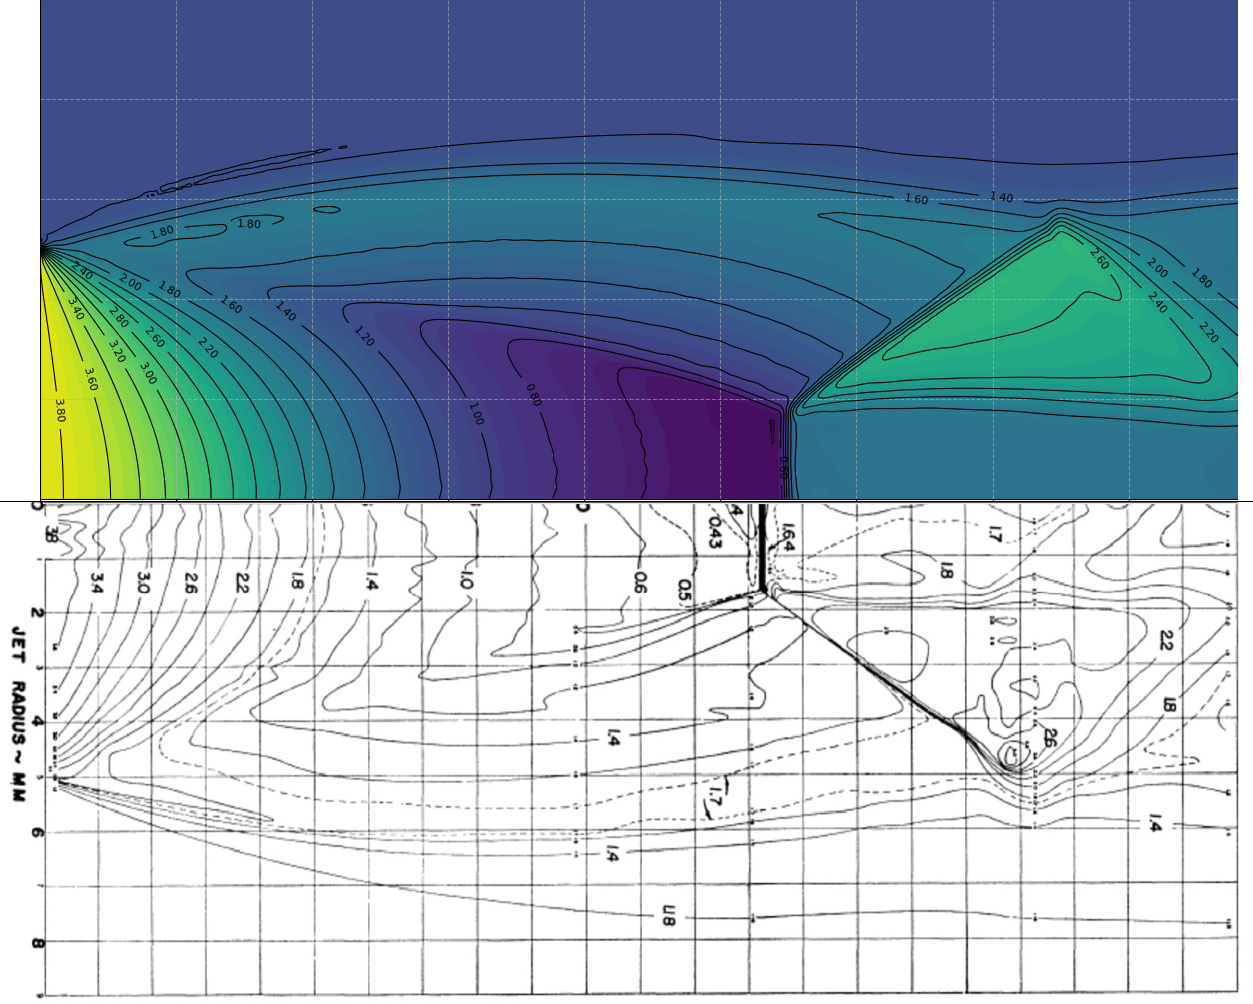
\includegraphics[width=0.83\linewidth]{figs/stacked_rho_OF_vs_EXP_viridis.png}
    \caption{Density distribution of the supersonic jet measured by Ladenburg~\cite{ladenburg1949interferometric} (lower of panel), and computational results (upper panel) obtained with OpenFOAM. %The values of the density contours are provided in $kg/m^3$.
    }
    \label{fig:rho_OF_vs_EXP_viridis}
\end{figure}
%
\vspace{-0.5cm}
%
%NEW
\begin{figure}[H]
    \centering
    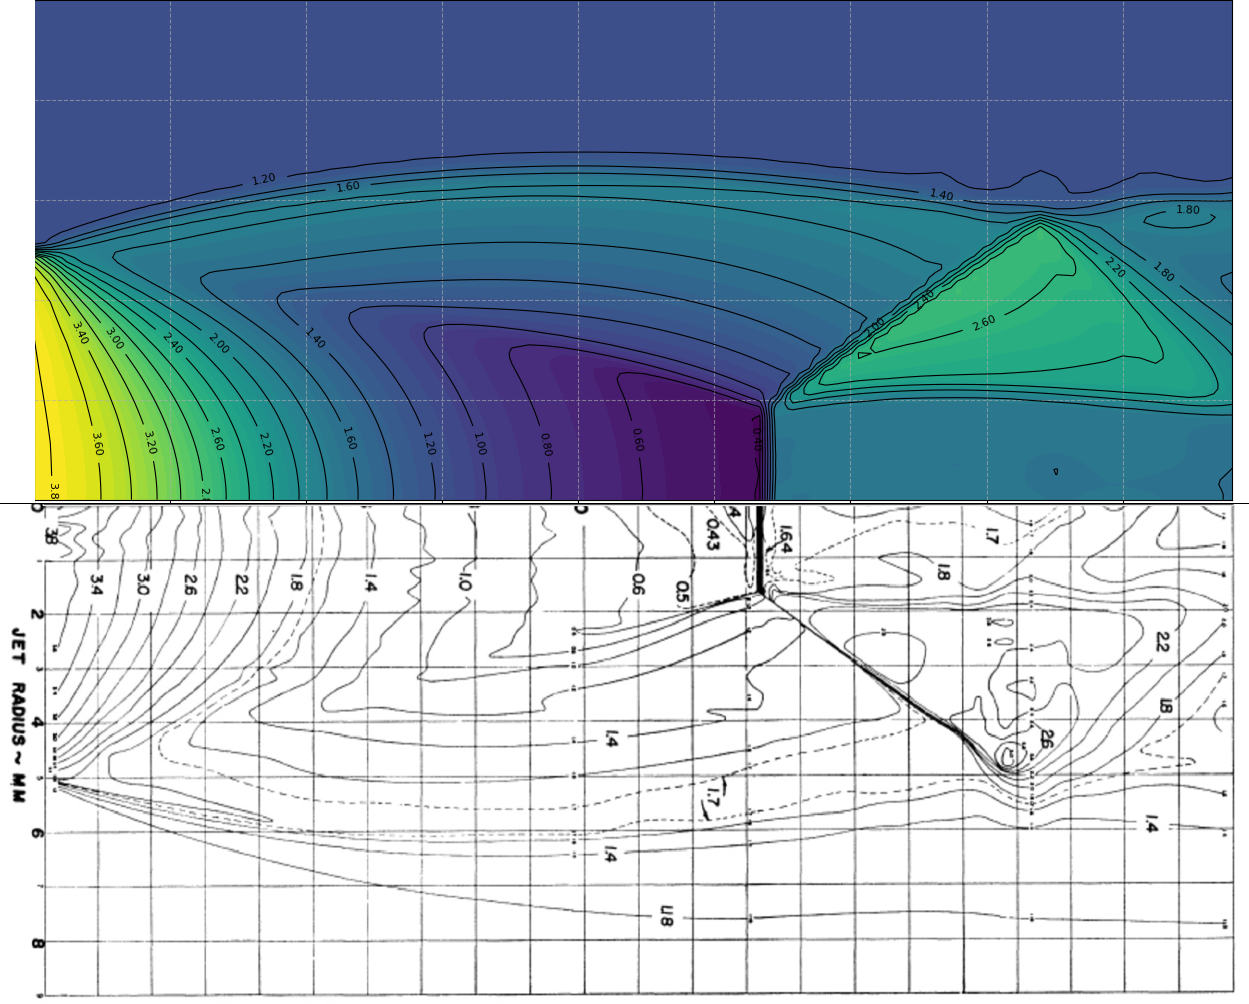
\includegraphics[width=0.83\linewidth]{figs/stacked_rho_FLUENT_vs_EXP_viridis.png}
    \caption{Density distribution of the supersonic jet measured by Ladenburg~\cite{ladenburg1949interferometric} (lower of panel), and computational results (upper panel) obtained with FLUENT. %The values of the density contours are provided in $kg/m^3$.
    }
    \label{fig:rho_FLUENT_vs_EXP_viridis}
\end{figure}

%NEW
\begin{figure}[H]
    \centering
    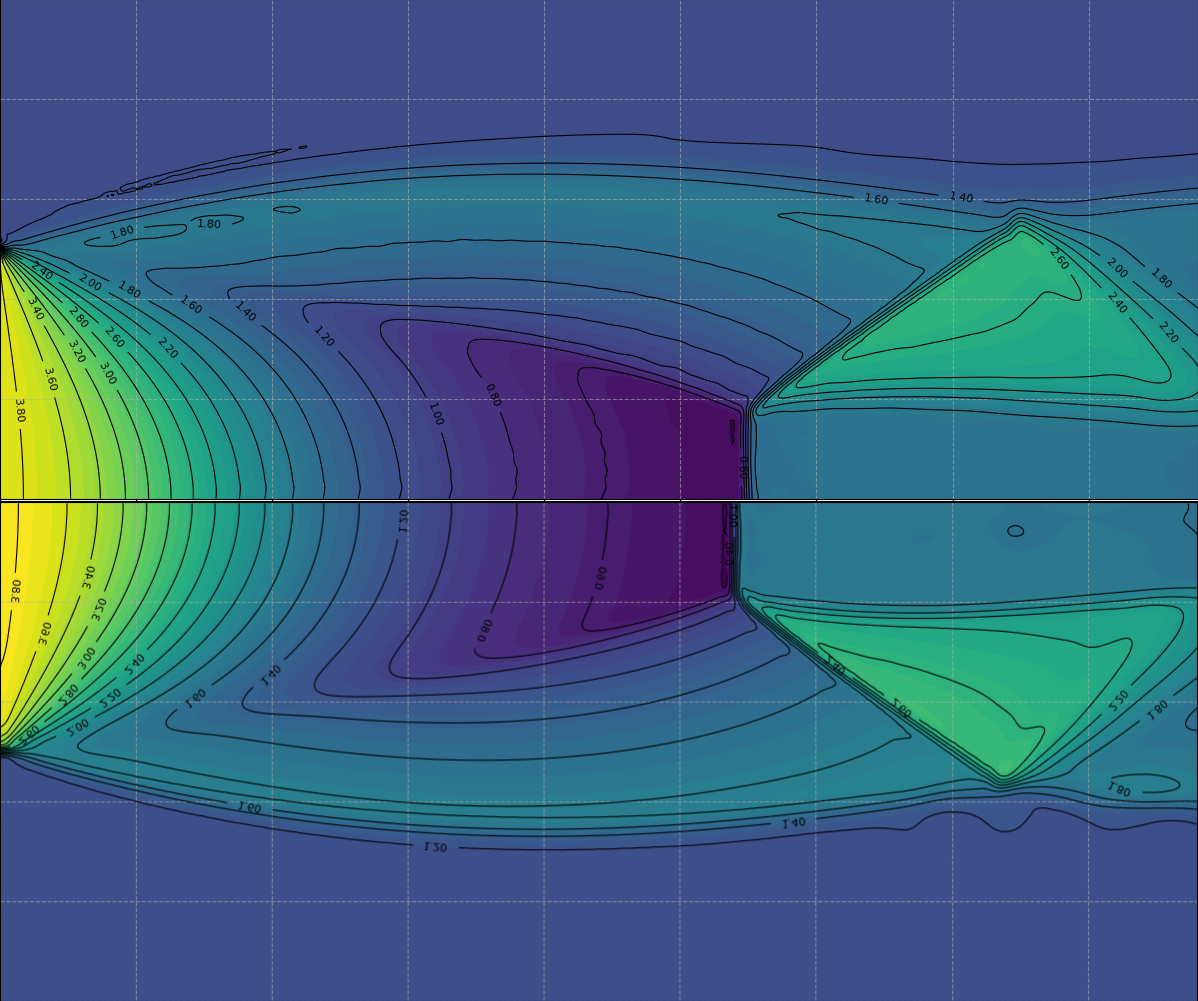
\includegraphics[width=\linewidth]{figs/stacked_rho_OF_vs_FLUENT_viridis.png}
    \caption{Density distribution of the supersonic jet computational results obtained with OpenFOAM (upper panel) and FLUENT (lower panel). %The values of the density contours are provided in $kg/m^3$.
    }
    \label{fig:rho_OF_vs_FLUENT_viridis}
\end{figure}

%%% other CFD results
\begin{figure}[H]
    \centering
    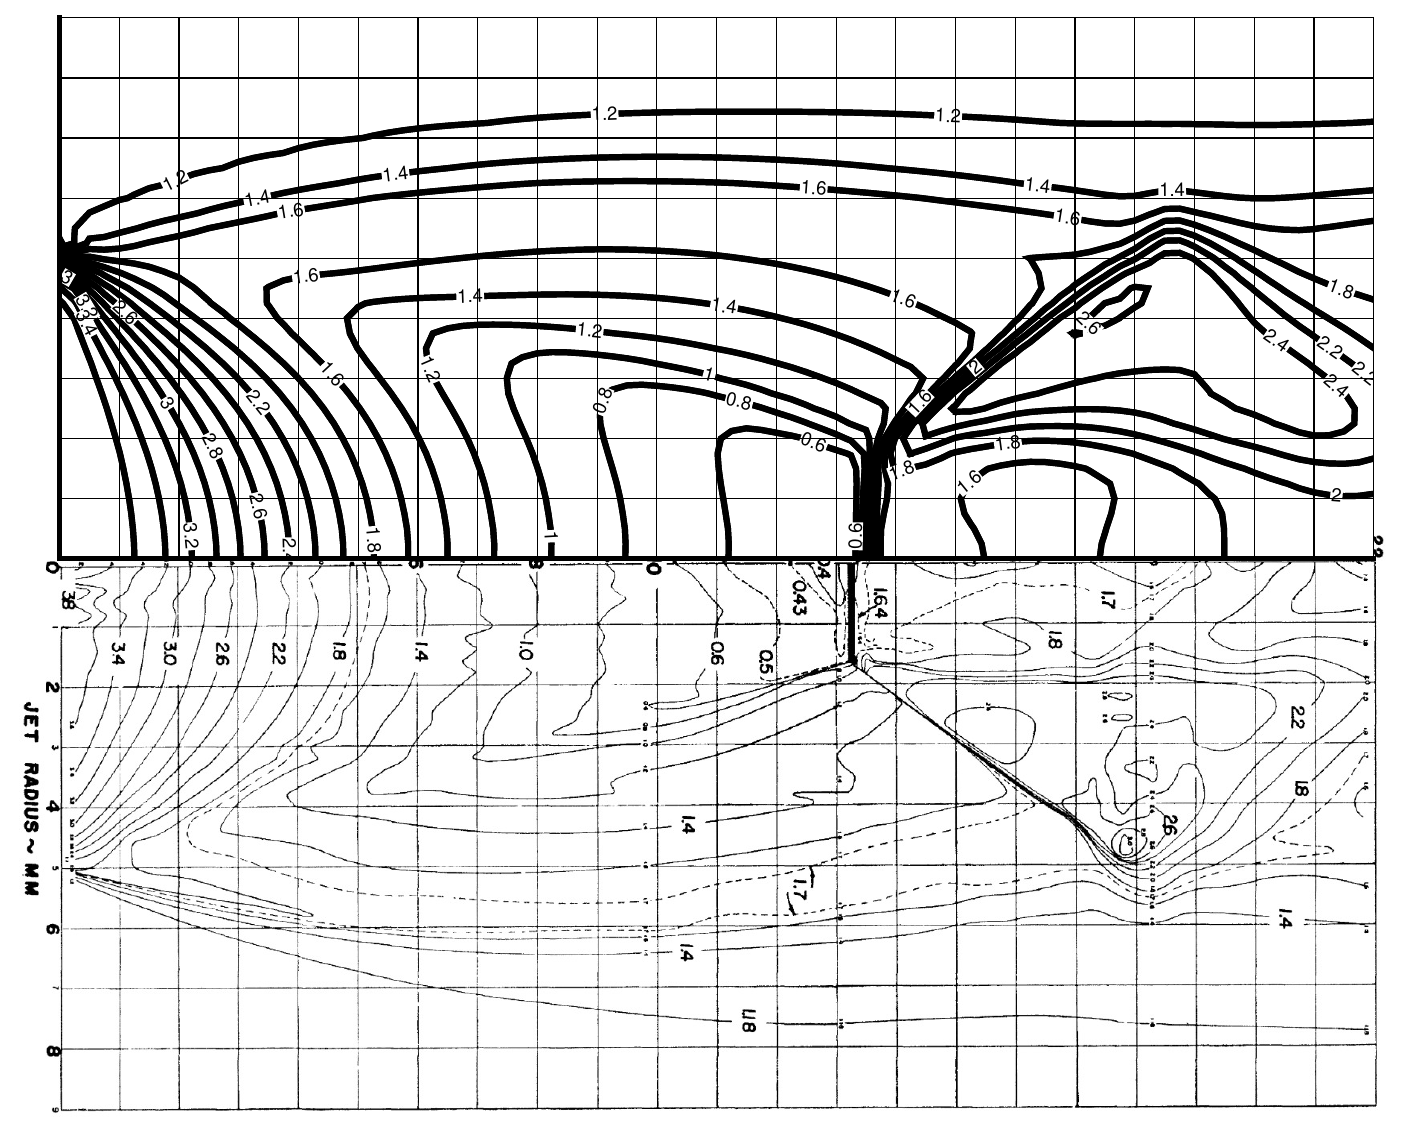
\includegraphics[width=0.775\linewidth]{figs/comp1.png}
    \caption{Density distribution of the supersonic jet measured by Ladenburg~\cite{ladenburg1949interferometric} (lower of panel), and computational results (upper panel) by \cite{kumar2021role}.%The values of the density contours are provided in $kg/m^3$.
    }
    \label{fig:comp1}
\end{figure}

\begin{figure}[H]
    \centering
    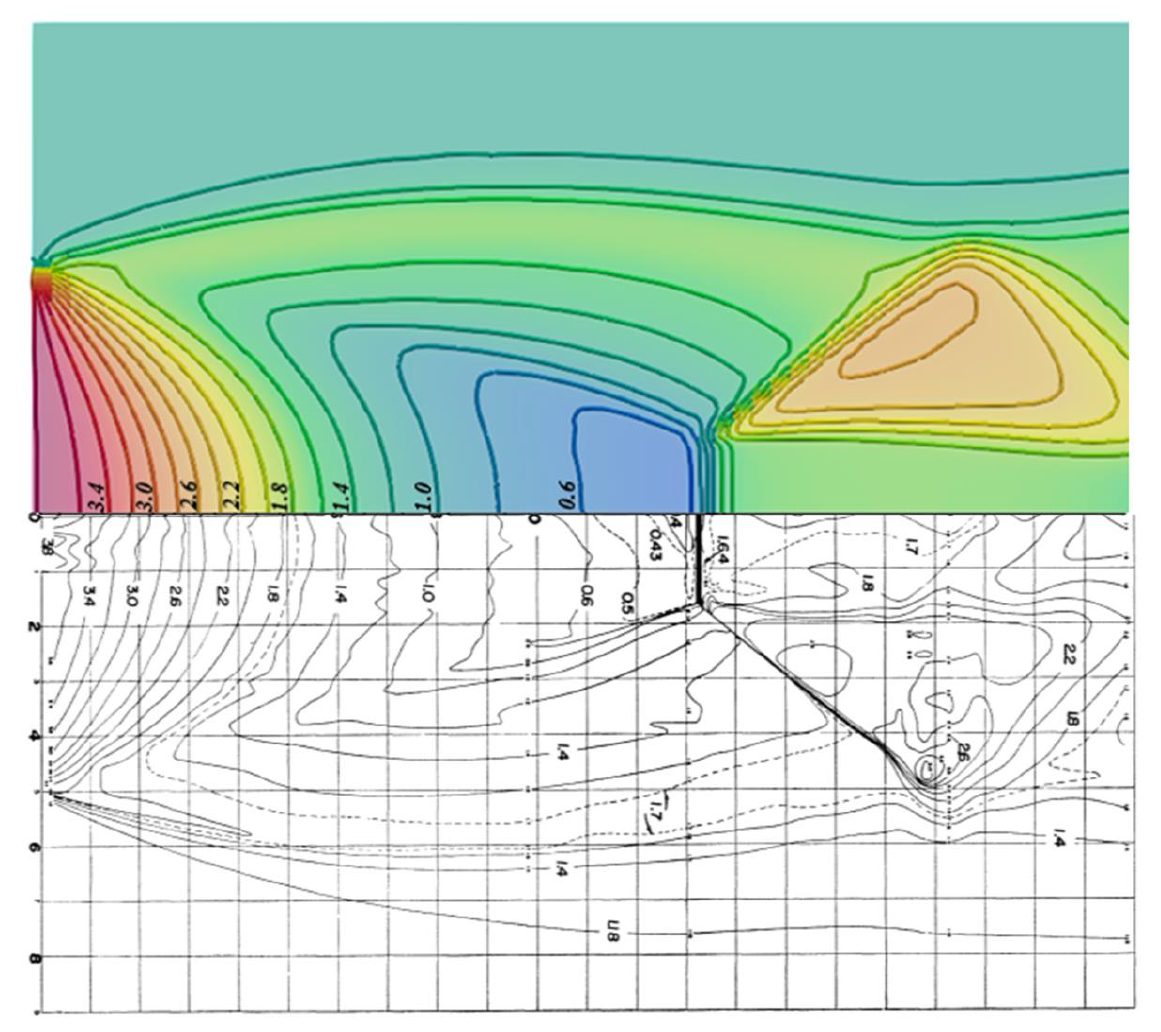
\includegraphics[width=0.775\linewidth]{figs/comp2.png}
    \caption{Density distribution of the supersonic jet measured by Ladenburg~\cite{ladenburg1949interferometric} (lower of panel), and computational results (upper panel) by \cite{gilmanov2024development}. %The values of the density contours are provided in $kg/m^3$.
    } 
    \label{fig:comp2}
\end{figure}

\begin{figure}[H]
    \centering
    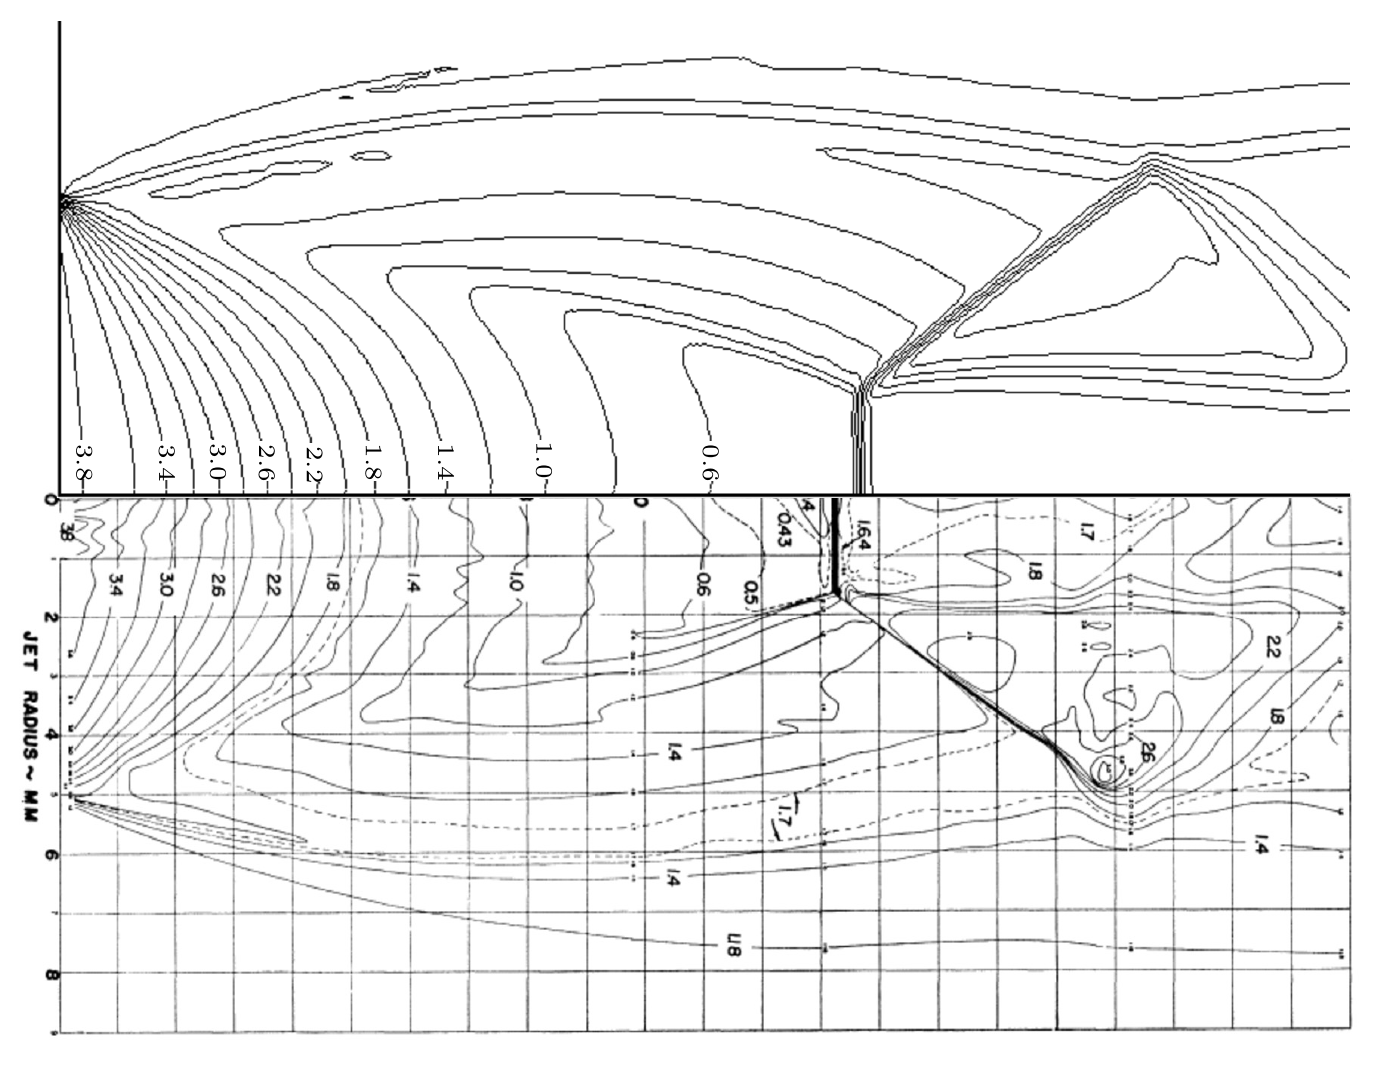
\includegraphics[width=0.95\linewidth]{figs/comp3.png}
    \caption{Density distribution of the supersonic jet measured by Ladenburg~\cite{ladenburg1949interferometric} (lower of panel), and computational results (upper panel) by \cite{greenshields2010implementation}. %The values of the density contours are provided in $kg/m^3$.
    }
    \label{fig:comp3}
\end{figure}

\newpage 

%%%%%%%%%%%%%%%%%%%%%%%%%%%%%%%%%%%%%%%%%%%%
\section{Conclusions}\label{sec:conclusions}
%%%%%%%%%%%%%%%%%%%%%%%%%%%%%%%%%%%%%%%%%%%%
In this work package, the Ladenburg jet test case~\cite{ladenburg1949interferometric} was  simulated with OpenFOAM and FLUENT solvers and numerical solutions were compared with the available experimental data. Among the key findings, it can be reported that:

\begin{itemize}
    \item The simulations reproduce the Mach disk location and triple point with acceptable accuracy and precision even if numerical solution present some offset respect to the experimental data.
    \item The simulations capture complex shock interactions (Mach reflections, barrel shocks) fairly satisfactorily.
    \item A fairly good agreement with experimental density and pressure contours and profile has been obtained by both solvers.
    \item A good agreement between the numerical solutions of both solvers was achieved for all considered variables and shock location.
    \item Numerical simulations manifest a proper treatment of expansion fans and shock wave interactions.
\end{itemize}

Some important aspect were omitted from the current work package, such as the effect of the turbulence model and grid refinement. In fact, the current numerical campaign assumed a laminar flow and no turbulence model was used. Moreover, the computational grids adopted a simple cartesian topology without adaptation, not even around boundary or shear layers.

Thanks to these results, an increased confidence in the OpenFOAM and FLUENT solvers was obtained. In particular, the influence of different boundary conditions was also partially assessed. The numerical simulation of the Charon jet-on configuration will rely on such confidence.

% Signature
\vspace{\fill}
\begin{center}
    \hspace*{9.0cm} \LARGE \textbf{Lorenzo Campoli} \\
    \hspace*{9.0cm}
\includegraphics[width=0.45\textwidth]{signature/signature0.png}
\end{center}

\vspace*{-1.0cm}

\hspace*{9.0cm}\textbf{Senior Systems Modelling Engineer}

\hspace*{9.0cm}\textbf{Gilmour Space Technologies}

\hspace*{9.0cm}\textbf{lorenzo.campoli@gspace.com}

\newpage
\bibliography{refs/refs}
\bibliographystyle{unsrt}

%\newpage % TODO
%\section*{Work in Progress}

\begin{description}
    \item[Checklists] to go through during peer review of the analysis.
\end{description}

\subsection*{Pre-setup Checks}
\begin{itemize}
    \item[$\checkmark$] Goals of the analysis defined.
    \item[$\checkmark$] All operating cases and conditions identified, both flight and ground if applicable.
    \item[$\checkmark$] Boundary and initial conditions identified and selected.
    \item[$\checkmark$] Required dimensionality of the spatial model understood (2D, full 3D, slice 3D).
    \item[$\checkmark$] Appropriate temporal modelling identified (steady or transient).
    \item[$\checkmark$] Made educated guess of what final results will look like.
    \item[$\checkmark$] Assumptions being made have been identified.
    \item[$\checkmark$] Remember that CFD should stand for Computational Fluid Dynamics and not Colours For Director!
\end{itemize}

\subsection*{Setup Checks}

\subsubsection*{Geometry and Mesh:}
\begin{itemize}
    \item[$\checkmark$] Geometry is at worst case tolerances.
    \item[$\checkmark$] Check the geometry is a watertight 3D solid or 2D surface.
    \item[$\checkmark$] Use descriptive strings to name entities (e.g. fluid, inlet, outlet, wall, axis, symmetry, periodicity).
    \item[$\checkmark$] If using a 2D axisymmetric model, check the axis of rotation is the x-axis of the model.
    \item[$\checkmark$] Choose suitable mesh type for low vs large cell count and simple vs complex geometries.
    \item[$\checkmark$] Select appropriate meshing methods, global controls, and local sizings.
    \item[$\checkmark$] If resolving directly the wall boundary layer is important, use inflation layers to achieve y+ ~ 1 (Fluent 2023 R2 Theory Guide 4.7.3).
    \item[$\checkmark$] If using wall functions, use inflation layers to achieve a y+ of an appropriate range for the specified near-wall treatment setting (Fluent 2023 R2 Theory Guide 4.17).
    \item[$\checkmark$] Assure a constant growth rate between inflation layers and volume mesh.
    \item[$\checkmark$] Check that in the regions of interest the mesh does not have high growth rate or large steps in mesh size such as octree transitions in hex mesh.
    \item[$\checkmark$] Check mesh quality metrics (e.g. orthogonal quality > 0.1, average skewness < 0.33, maximum skewness < 0.85) (Fluent 2023 R2 User's Guide II.5.3 and III.6.2).
    \item[$\checkmark$] Mesh passes fluent mesh check.
\end{itemize}

\subsubsection*{Physics Models and Boundary Conditions:}
\begin{itemize}
    \item[$\checkmark$] Select the suitable physics models.
    \item[$\checkmark$] Use the appropriate turbulence model (k-w SST industry standard for several problems). Consider activating curvature correction for swirling flows.
    \item[$\checkmark$] Double check material properties.
    \item[$\checkmark$] Ideal or real fluid properties properly defined and sources documented for new properties entered.
    \item[$\checkmark$] Correct units used for all boundary condition inputs.
    \item[$\checkmark$] Reference quantities set appropriately.
    \item[$\checkmark$] Operating pressure set appropriately to avoid roundoff error problems (Fluent 2023 R2 User's Guide III.8.14). Where no pressure boundary conditions are used, reference pressure location has been set (Fluent 2023 R2 User's Guide III.8.15).
    \item[$\checkmark$] Pressures are all input as gauge wrt the operating pressure.
    \item[$\checkmark$] Gravity set correctly if needed.
\end{itemize}

\subsubsection*{Numerical Methods and Solution Controls:}
\begin{itemize}
    \item[$\checkmark$] Considered if the single or double precision solver is needed (Fluent User's Guide I.4.1.2.2).
    \item[$\checkmark$] Choose the appropriate solver type and temporal model.
    \item[$\checkmark$] Use 2nd order schemes if possible.
    \item[$\checkmark$] Adjust absolute convergence criteria for residuals (e.g. to 1E-6).
    \item[$\checkmark$] Define suitable report definitions and monitors.
    \item[$\checkmark$] Autosave data file every XXX iterations to preserve results and retain only the most recent files.
\end{itemize}

\subsection*{Results}
\begin{longtable}{|c|c|c|}
    \hline
    Case & Key result 1 & Key result 2 \\
    \hline
    \endfirsthead
    \hline
    Case & Key result 1 & Key result 2 \\
    \hline
    \endhead
    \hline
    \endfoot
    \hline
    Case 1 & Value 1 & Value 2 \\
    Case 2 & Value 1 & Value 2 \\
\end{longtable}

\noindent Concise presentation of findings with screenshots only of crucial parts.

\noindent Comparison to analytical methods or sanity checks.

\noindent Add table of sensitivity to assumptions if applicable.

\subsection*{Mesh Independence Check}
\begin{longtable}{|c|c|c|c|}
    \hline
    Case & \# of elements & Change in key result 1 & Change in key result 2 \\
    \hline
    \endfirsthead
    \hline
    Case & \# of elements & Change in key result 1 & Change in key result 2 \\
    \hline
    \endhead
    \hline
    \endfoot
    \hline
    Case 1 & 1000 & 0.01 & 0.02 \\
    Case 2 & 2000 & 0.005 & 0.01 \\
\end{longtable}

\newpage

\section*{Goals}
\begin{itemize}
    \item \textbf{What are you analysing (and which locations are important)?}
    \item \textbf{Why are you doing it (Pressure losses estimate, prior to manufacture, trade study)?}
    \item \textbf{How much accuracy is needed?}
    \item \textbf{Does this need CFD or could it be done with analytical methods, or testing?}
\end{itemize}

\section*{Geometry and Mesh}
\begin{itemize}
    \item \textbf{Screenshot of geometry.}
    \item \textbf{Screenshot of typical mesh and refined regions.}
    \item \textbf{Key mesh sizing.}
    \item \textbf{Overall mesh quality.}
    \item \textbf{Total number of elements.}
\end{itemize}

\section*{Physics Model and Boundary Conditions}
\begin{itemize}
    \item \textbf{Include annotated screenshots as required.}
\end{itemize}

\section*{Numerical Methods and Solution Controls}
\begin{itemize}
    \item \textbf{Solver settings details screenshot.}
\end{itemize}

\newpage

\section{Appendix}
%%%%%%%%%%%%%%%%%%
The Python code snippet in Listing~\ref{lst:ppost} was used to generate contour plot flow images and solution ASCII data to be further post-processed and then incorporated in the current report. The script was imported in Paraview as macro and executed upon the raw solution file was loaded directly from within. Note that it could also run in batch mode from command line.

\begin{lstlisting}[language=python, caption=Script for the generation of images and data from the CFD results., label=lst:ppost]
# trace generated using paraview version 5.10.0-RC1
#import paraview
#paraview.compatibility.major = 5
#paraview.compatibility.minor = 10

#### import the simple module from the paraview
from paraview.simple import *
#### disable automatic camera reset on 'Show'
paraview.simple._DisableFirstRenderCameraReset()

# get active source.
g0foam = GetActiveSource()

# get active view
renderView1 = GetActiveViewOrCreate('RenderView')

# show data in view
g0foamDisplay = Show(g0foam, renderView1, 'UnstructuredGridRepresentation')

# get color transfer function/color map for 'p'
pLUT = GetColorTransferFunction('p')

# get opacity transfer function/opacity map for 'p'
pPWF = GetOpacityTransferFunction('p')

# trace defaults for the display properties.
g0foamDisplay.Representation = 'Surface'
g0foamDisplay.ColorArrayName = ['POINTS', 'p']
g0foamDisplay.LookupTable = pLUT
g0foamDisplay.SelectTCoordArray = 'None'
g0foamDisplay.SelectNormalArray = 'None'
g0foamDisplay.SelectTangentArray = 'None'
g0foamDisplay.OSPRayScaleArray = 'p'
g0foamDisplay.OSPRayScaleFunction = 'PiecewiseFunction'
g0foamDisplay.SelectOrientationVectors = 'U'
g0foamDisplay.ScaleFactor = 0.002999999932944775
g0foamDisplay.SelectScaleArray = 'p'
g0foamDisplay.GlyphType = 'Arrow'
g0foamDisplay.GlyphTableIndexArray = 'p'
g0foamDisplay.GaussianRadius = 0.00014999999664723872
g0foamDisplay.SetScaleArray = ['POINTS', 'p']
g0foamDisplay.ScaleTransferFunction = 'PiecewiseFunction'
g0foamDisplay.OpacityArray = ['POINTS', 'p']
g0foamDisplay.OpacityTransferFunction = 'PiecewiseFunction'
g0foamDisplay.DataAxesGrid = 'GridAxesRepresentation'
g0foamDisplay.PolarAxes = 'PolarAxesRepresentation'
g0foamDisplay.ScalarOpacityFunction = pPWF
g0foamDisplay.ScalarOpacityUnitDistance = 0.0029758189580041195
g0foamDisplay.OpacityArrayName = ['POINTS', 'p']

# init the 'PiecewiseFunction' selected for 'ScaleTransferFunction'
g0foamDisplay.ScaleTransferFunction.Points = [7809.06787109375, 0.0, 0.5, 0.0, 271724.0, 1.0, 0.5, 0.0]

# init the 'PiecewiseFunction' selected for 'OpacityTransferFunction'
g0foamDisplay.OpacityTransferFunction.Points = [7809.06787109375, 0.0, 0.5, 0.0, 271724.0, 1.0, 0.5, 0.0]

# reset view to fit data
renderView1.ResetCamera(False)

# show color bar/color legend
g0foamDisplay.SetScalarBarVisibility(renderView1, True)

# update the view to ensure updated data information
renderView1.Update()

# set scalar coloring
ColorBy(g0foamDisplay, ('POINTS', 'T'))

# Hide the scalar bar for this color map if no visible data is colored by it.
HideScalarBarIfNotNeeded(pLUT, renderView1)

# rescale color and/or opacity maps used to include current data range
g0foamDisplay.RescaleTransferFunctionToDataRange(True, False)

# show color bar/color legend
g0foamDisplay.SetScalarBarVisibility(renderView1, True)

# get color transfer function/color map for 'T'
tLUT = GetColorTransferFunction('T')

# get opacity transfer function/opacity map for 'T'
tPWF = GetOpacityTransferFunction('T')

# hide color bar/color legend
g0foamDisplay.SetScalarBarVisibility(renderView1, False)

# Properties modified on renderView1
renderView1.OrientationAxesVisibility = 0

# reset view to fit data
renderView1.ResetCamera(True)

# get layout
layout1 = GetLayout()

# layout/tab size in pixels
layout1.SetSize(1542, 784)

# current camera placement for renderView1
renderView1.CameraPosition = [0.014999999664723873, 0.004999999888241291, 0.06109054909012853]
renderView1.CameraFocalPoint = [0.014999999664723873, 0.004999999888241291, 0.0]
renderView1.CameraViewAngle = 15.520968439256377
renderView1.CameraParallelScale = 0.015811397580295733

# save screenshot
SaveScreenshot('./T.png', renderView1, ImageResolution=[1542, 784],
    TransparentBackground=1)

# set scalar coloring
ColorBy(g0foamDisplay, ('POINTS', 'U', 'Magnitude'))

# Hide the scalar bar for this color map if no visible data is colored by it.
HideScalarBarIfNotNeeded(tLUT, renderView1)

# rescale color and/or opacity maps used to include current data range
g0foamDisplay.RescaleTransferFunctionToDataRange(True, False)

# show color bar/color legend
g0foamDisplay.SetScalarBarVisibility(renderView1, True)

# get color transfer function/color map for 'U'
uLUT = GetColorTransferFunction('U')

# get opacity transfer function/opacity map for 'U'
uPWF = GetOpacityTransferFunction('U')

# hide color bar/color legend
g0foamDisplay.SetScalarBarVisibility(renderView1, False)

# layout/tab size in pixels
layout1.SetSize(1542, 784)

# current camera placement for renderView1
renderView1.CameraPosition = [0.014999999664723873, 0.004999999888241291, 0.06109054909012853]
renderView1.CameraFocalPoint = [0.014999999664723873, 0.004999999888241291, 0.0]
renderView1.CameraViewAngle = 15.520968439256377
renderView1.CameraParallelScale = 0.015811397580295733

# save screenshot
SaveScreenshot('./U.png', renderView1, ImageResolution=[1542, 784],
    TransparentBackground=1)

# set scalar coloring
ColorBy(g0foamDisplay, ('POINTS', 'p'))

# Hide the scalar bar for this color map if no visible data is colored by it.
HideScalarBarIfNotNeeded(uLUT, renderView1)

# rescale color and/or opacity maps used to include current data range
g0foamDisplay.RescaleTransferFunctionToDataRange(True, False)

# show color bar/color legend
g0foamDisplay.SetScalarBarVisibility(renderView1, True)

# hide color bar/color legend
g0foamDisplay.SetScalarBarVisibility(renderView1, False)

# layout/tab size in pixels
layout1.SetSize(1542, 784)

# current camera placement for renderView1
renderView1.CameraPosition = [0.014999999664723873, 0.004999999888241291, 0.06109054909012853]
renderView1.CameraFocalPoint = [0.014999999664723873, 0.004999999888241291, 0.0]
renderView1.CameraViewAngle = 15.520968439256377
renderView1.CameraParallelScale = 0.015811397580295733

# save screenshot
SaveScreenshot('./p.png', renderView1, ImageResolution=[1542, 784],
    TransparentBackground=1)

# set scalar coloring
ColorBy(g0foamDisplay, ('POINTS', 'rho'))

# Hide the scalar bar for this color map if no visible data is colored by it.
HideScalarBarIfNotNeeded(pLUT, renderView1)

# rescale color and/or opacity maps used to include current data range
g0foamDisplay.RescaleTransferFunctionToDataRange(True, False)

# show color bar/color legend
g0foamDisplay.SetScalarBarVisibility(renderView1, True)

# get color transfer function/color map for 'rho'
rhoLUT = GetColorTransferFunction('rho')

# get opacity transfer function/opacity map for 'rho'
rhoPWF = GetOpacityTransferFunction('rho')

# hide color bar/color legend
g0foamDisplay.SetScalarBarVisibility(renderView1, False)

# layout/tab size in pixels
layout1.SetSize(1542, 784)

# current camera placement for renderView1
renderView1.CameraPosition = [0.014999999664723873, 0.004999999888241291, 0.06109054909012853]
renderView1.CameraFocalPoint = [0.014999999664723873, 0.004999999888241291, 0.0]
renderView1.CameraViewAngle = 15.520968439256377
renderView1.CameraParallelScale = 0.015811397580295733

# save screenshot
SaveScreenshot('./rho.png', renderView1, ImageResolution=[1542, 784],
    TransparentBackground=1)

# destroy renderView1
Delete(renderView1)
del renderView1

# Create a new 'SpreadSheet View'
spreadSheetView1 = CreateView('SpreadSheetView')
spreadSheetView1.ColumnToSort = ''
spreadSheetView1.BlockSize = 1024

# show data in view
g0foamDisplay = Show(g0foam, spreadSheetView1, 'SpreadSheetRepresentation')

# assign view to a particular cell in the layout
AssignViewToLayout(view=spreadSheetView1, layout=layout1, hint=0)

# export view
ExportView('./solution.csv', view=spreadSheetView1)

SelectCompositeDataIDs(IDs=[1, -1, 9], FieldType=1, ContainingCells=0)

# set active source
SetActiveSource(g0foam)
\end{lstlisting}

\end{document}